\documentclass[11pt,a4paper]{article}

\usepackage[T1]{fontenc}
\usepackage{lmodern}
\usepackage[margin=2.4cm]{geometry}
\usepackage{graphicx}
\usepackage{booktabs}
\usepackage{array}
\usepackage{amsmath}
\usepackage{caption}
\usepackage{float}
\usepackage{xcolor}
\usepackage{enumitem}
\usepackage{microtype}
\usepackage[colorlinks=true,linkcolor=blue!50!black,citecolor=blue!50!black,urlcolor=blue!50!black]{hyperref}
\graphicspath{{figures/}}
\captionsetup{font=small,labelfont=bf}
\setlength{\parskip}{4pt}
\setlength{\parindent}{0pt}
\renewcommand{\arraystretch}{1.12}

\title{\textbf{Four YOLO Small Detectors on a 204-Photograph Custom Dataset:\\ What a 21-Image Test Set Can and Cannot Tell Us}}
\author{Tanjim Samad Swapnil\\[2pt]
{\small Mechatronics Engineering, Rajshahi University of Engineering \& Technology (RUET), Bangladesh}}
\date{10 November 2026}

\begin{document}
\maketitle

\begin{abstract}
\noindent Small custom datasets are normal in industrial inspection, yet results on them are often read as if the test split were large. I trained YOLOv8s, YOLO11s, YOLO12s and YOLO26s with one fixed recipe (COCO-pretrained weights, AdamW, batch size 4, 640~px, online augmentation switched off) on 489 Roboflow-augmented images that come from 163 photographs of a packaged-medicine carton labelled \emph{Good} or \emph{Miss\_Print}, and evaluated them once on 21 further photographs holding 29 boxes. Test mAP@50:95 ranged from 0.583 (YOLOv8s) to 0.727 (YOLO12s); mAP@50 ranged from 0.858 to 0.960. An image-level bootstrap put 95\,\% intervals about $\pm$0.1 wide around every mAP@50:95. YOLO12s and YOLO26s could not be separated (difference 0.035, interval $-$0.022 to $+$0.099), nor could YOLOv8s and YOLO11s, whereas both newer models exceeded both older ones. Training box loss fell from about 1.5 to 0.11--0.29 while validation box loss never fell below 0.95 and reached 1.5--2.1 at its worst, and the best checkpoint came as early as epoch 8 of 33. Two of the four models lost 0.09--0.12 of validation mAP@50:95 within 25 epochs after their peak, the other two 0.02--0.04. The evidence supports a hypothesis that the two newer architectures overfit less on this dataset; it does not establish a ranking. The report explains why, lists what was not tested, and gives a prioritised plan to turn the hypothesis into a result. All code, logs, figures and weights are in the accompanying repository.
\end{abstract}

\section{Introduction}
A bounding-box detector for a production-line check is often trained on a few hundred photographs taken by the person who will deploy it. The data are expensive in time rather than money, the defect class is rare or hand-made, and a published benchmark for the exact product does not exist. Two habits then cause trouble. The first is to report a single mAP from a handful of test images with four decimals, which suggests a precision the sample cannot support. The second is to treat falling training loss as progress.

This project compares four recent members of the Ultralytics YOLO family on one such dataset. The question was practical: which of YOLOv8s, YOLO11s, YOLO12s and YOLO26s should be used for a two-class carton-print inspection task? The answer turned out to depend less on the architectures than on how little the data can distinguish between them. The contributions are therefore methodological and descriptive:
\begin{itemize}[leftmargin=1.4em,itemsep=1pt]
  \item an audited description of the dataset, showing that 489 training files represent 163 independent photographs and that validation and test contain 20 and 21 photographs with no photograph shared between splits (Section~\ref{sec:data});
  \item a four-way comparison under an identical recipe, with per-class results, training dynamics and an operating-point error count (Section~\ref{sec:results});
  \item image-level bootstrap intervals and paired model differences for the test metrics, which show which parts of the ranking survive resampling and which do not (Section~\ref{sec:uncertainty});
  \item an evidence-linked explanation of why a dataset of this size fails to support firm conclusions and why the detectors overfit it (Section~\ref{sec:why}), followed by what was not tested and what to do next (Sections~\ref{sec:limits}--\ref{sec:next}).
\end{itemize}
No claim is made that these four models are ranked correctly in general; the experiment has one training run per model and one product.

\section{Background}
\subsection{The four detectors}
All four are single-stage, anchor-free detectors from the Ultralytics code base \cite{ultralytics_software}, descended from the original YOLO formulation \cite{redmon2015yolo}. Table~\ref{tab:models} lists the published facts that matter for this comparison. YOLO11 replaces the C2f blocks of YOLOv8 with C3k2 blocks and adds a spatial-attention module (C2PSA) to the backbone \cite{ultralytics_yolo11_vs_v8}. YOLOv12 centres the network on attention: area attention, a residual aggregation block (R-ELAN), FlashAttention, no positional encoding and a 7$\times$7 separable convolution as position perceiver; its authors report that FlashAttention limits it to recent NVIDIA GPU generations \cite{tian2025yolov12}. YOLO26 removes distribution focal loss, offers an NMS-free one-to-one head, trains with a hybrid SGD--Muon optimiser (MuSGD) and adds ProgLoss and a small-target-aware label assignment (STAL) \cite{ultralytics_yolo26_vs_11,chakrabarty2026yolo26}. The only independent account of YOLO26 that I found is itself a secondary review of Ultralytics material \cite{chakrabarty2026yolo26}, so its architectural description rests on the vendor's documentation.

\begin{table}[H]
\centering\small
\begin{tabular}{lcccl}
\toprule
Model & Params (M) & FLOPs (B) & COCO mAP$_{50:95}$ & Source of the three numbers\\
\midrule
YOLOv8s  & 11.2 & 28.6 & 44.9 & Ultralytics docs \cite{ultralytics_yolo11_vs_v8}\\
YOLO11s  & 9.4  & 21.6 & 47.0 & Ultralytics docs \cite{ultralytics_yolo11_vs_v8}\\
YOLOv12-S & 9.3 & 21.4 & 48.0 & original paper \cite{tian2025yolov12}\\
YOLO26s  & 9.5  & 20.9 & 48.6 & Ultralytics docs \cite{ultralytics_yolo26_vs_11}\\
\bottomrule
\end{tabular}
\caption{Published COCO figures at 640~px for the four checkpoints. The rows come from different documents and evaluation set-ups, so they should not be subtracted from each other. The notebook's model summaries list about 11.14, 9.43, 9.25 and 9.95~M parameters for the unfused models (the last figure, for YOLO26s, is above the documented 9.5~M; a 9.47~M summary also appears, probably the fused model, and I did not trace this further).}
\label{tab:models}
\end{table}

\subsection{Why small datasets fail}
Four well-documented effects apply directly here. (i)~\emph{Memorisation is cheap.} Networks of this class can fit random labels on training images \cite{zhang2017rethinking}, so a low training loss does not show that anything general was learned. (ii)~\emph{Deep networks rely on data volume to avoid overfitting}, and augmentation is the standard remedy \cite{shorten2019survey}. (iii)~\emph{Pretraining helps but is not a regulariser.} On COCO subsets, training from scratch broke down between roughly 3.5k and 10k images, whereas pretrained models still worked at 1k images (9.9 versus 3.5 AP); the same paper reports that pretraining overfit on a 35k-image subset under unchanged hyper-parameters and states that pretraining does not necessarily provide regularisation \cite{he2019rethinking}. (iv)~\emph{Test-set size limits what a benchmark can resolve.} Variance from data sampling is well explained by the limited statistical power of the test set, and the authors recommend resampling over a single fixed held-out set \cite{bouthillier2021variance}. Ultralytics' own guidance, written for YOLOv5 but still the vendor's training advice, asks for at least 1\,500 images and 10\,000 labelled instances per class \cite{ultralytics_tips}. This project has 371 and 306 training instances.

\section{Dataset and audit}\label{sec:data}
The images were photographed and annotated with bounding boxes in Roboflow (project \texttt{Fault\_Detection\_Model}, version 2). Four exports of the same project (YOLOv8, YOLO11, YOLO12 and YOLO26 formats) were downloaded; SHA-256 hashes of every image and label file were identical across the four, so one copy was used (1\,060 files: 530 images and 530 label files). A validation script rejected unknown class ids, coordinates outside $[0,1]$ and degenerate boxes, and converted six polygon labels in the training split to enclosing boxes. Every image is 640$\times$640 pixels.

\begin{table}[H]
\centering\small
\begin{tabular}{lcccc}
\toprule
Split & Photographs$^{*}$ & Images & Boxes & Good / Miss\_Print\\
\midrule
Train & 163 & 489 & 677 & 371 / 306\\
Valid & 20 & 20 & 27 & 15 / 12\\
Test  & 21 & 21 & 29 & 14 / 15\\
\bottomrule
\end{tabular}
\caption{Dataset composition. $^{*}$Counted from the file-name stem before Roboflow's \texttt{.rf.} hash: 163 distinct stems in training with at most three files each, and one file per stem in validation and test. No stem occurs in two splits and no byte-identical image occurs in two splits (checked by MD5).}
\label{tab:data}
\end{table}

Two facts from this audit shape everything that follows. First, the training split is a threefold offline augmentation of 163 photographs (489 $=$ 3$\times$163), so the effective number of independent training scenes is 163, not 489. Roboflow documents that offline augmentation is applied to training images only, which matches what I found \cite{roboflow_augmentation}; sampled training images show rotation with black borders and speckle noise. Second, the validation and test splits are tiny: a single missed box changes recall by 3.7 points on validation and 3.4 on test. About 0.16 of the image area is covered by the median box (0.019 to 0.96 range), so objects are large and mostly isolated; 8 of 21 test images contain two boxes.

\begin{figure}[H]
\centering
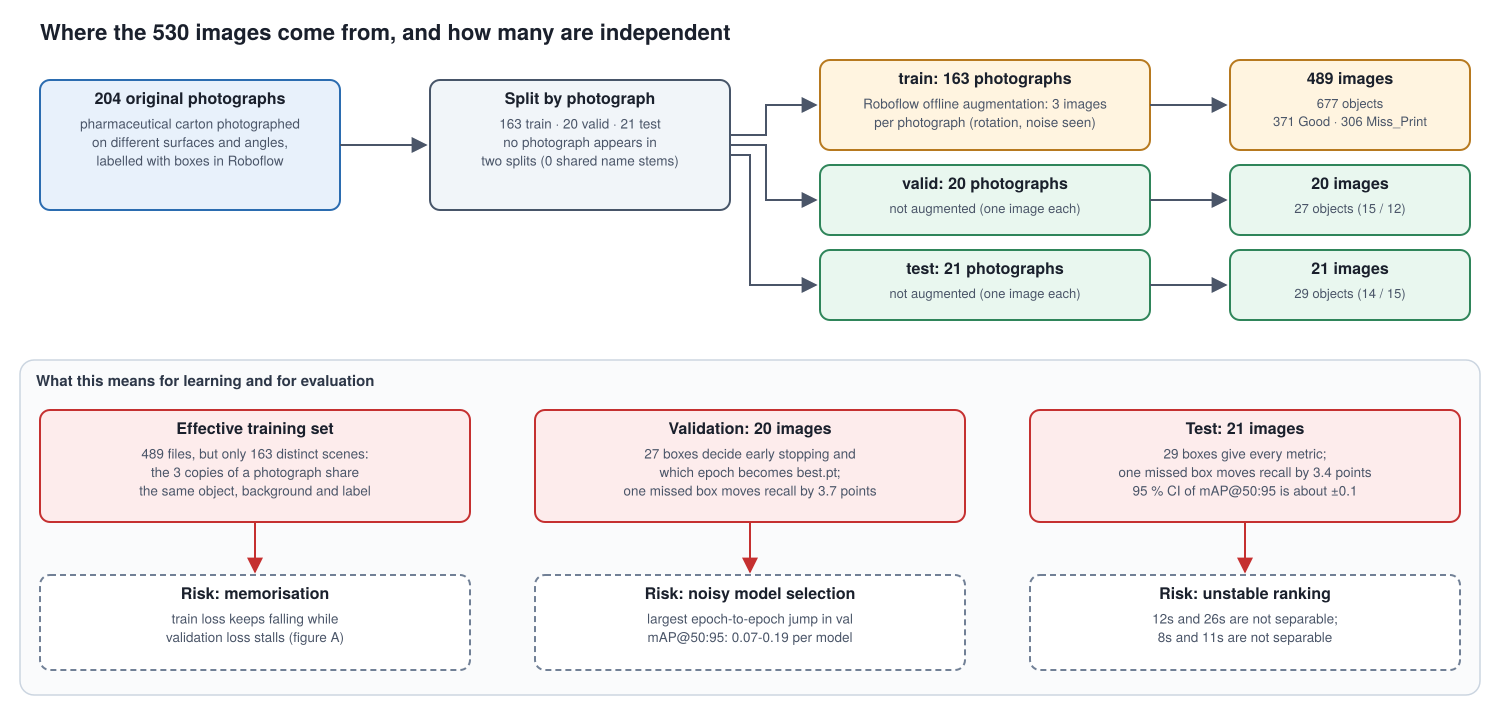
\includegraphics[width=\textwidth]{02_dataset_split_augmentation.png}
\caption{Where the 530 images come from and what the split sizes imply. Photograph counts are inferred from file names.}
\label{fig:dataflow}
\end{figure}

\begin{figure}[H]
\centering
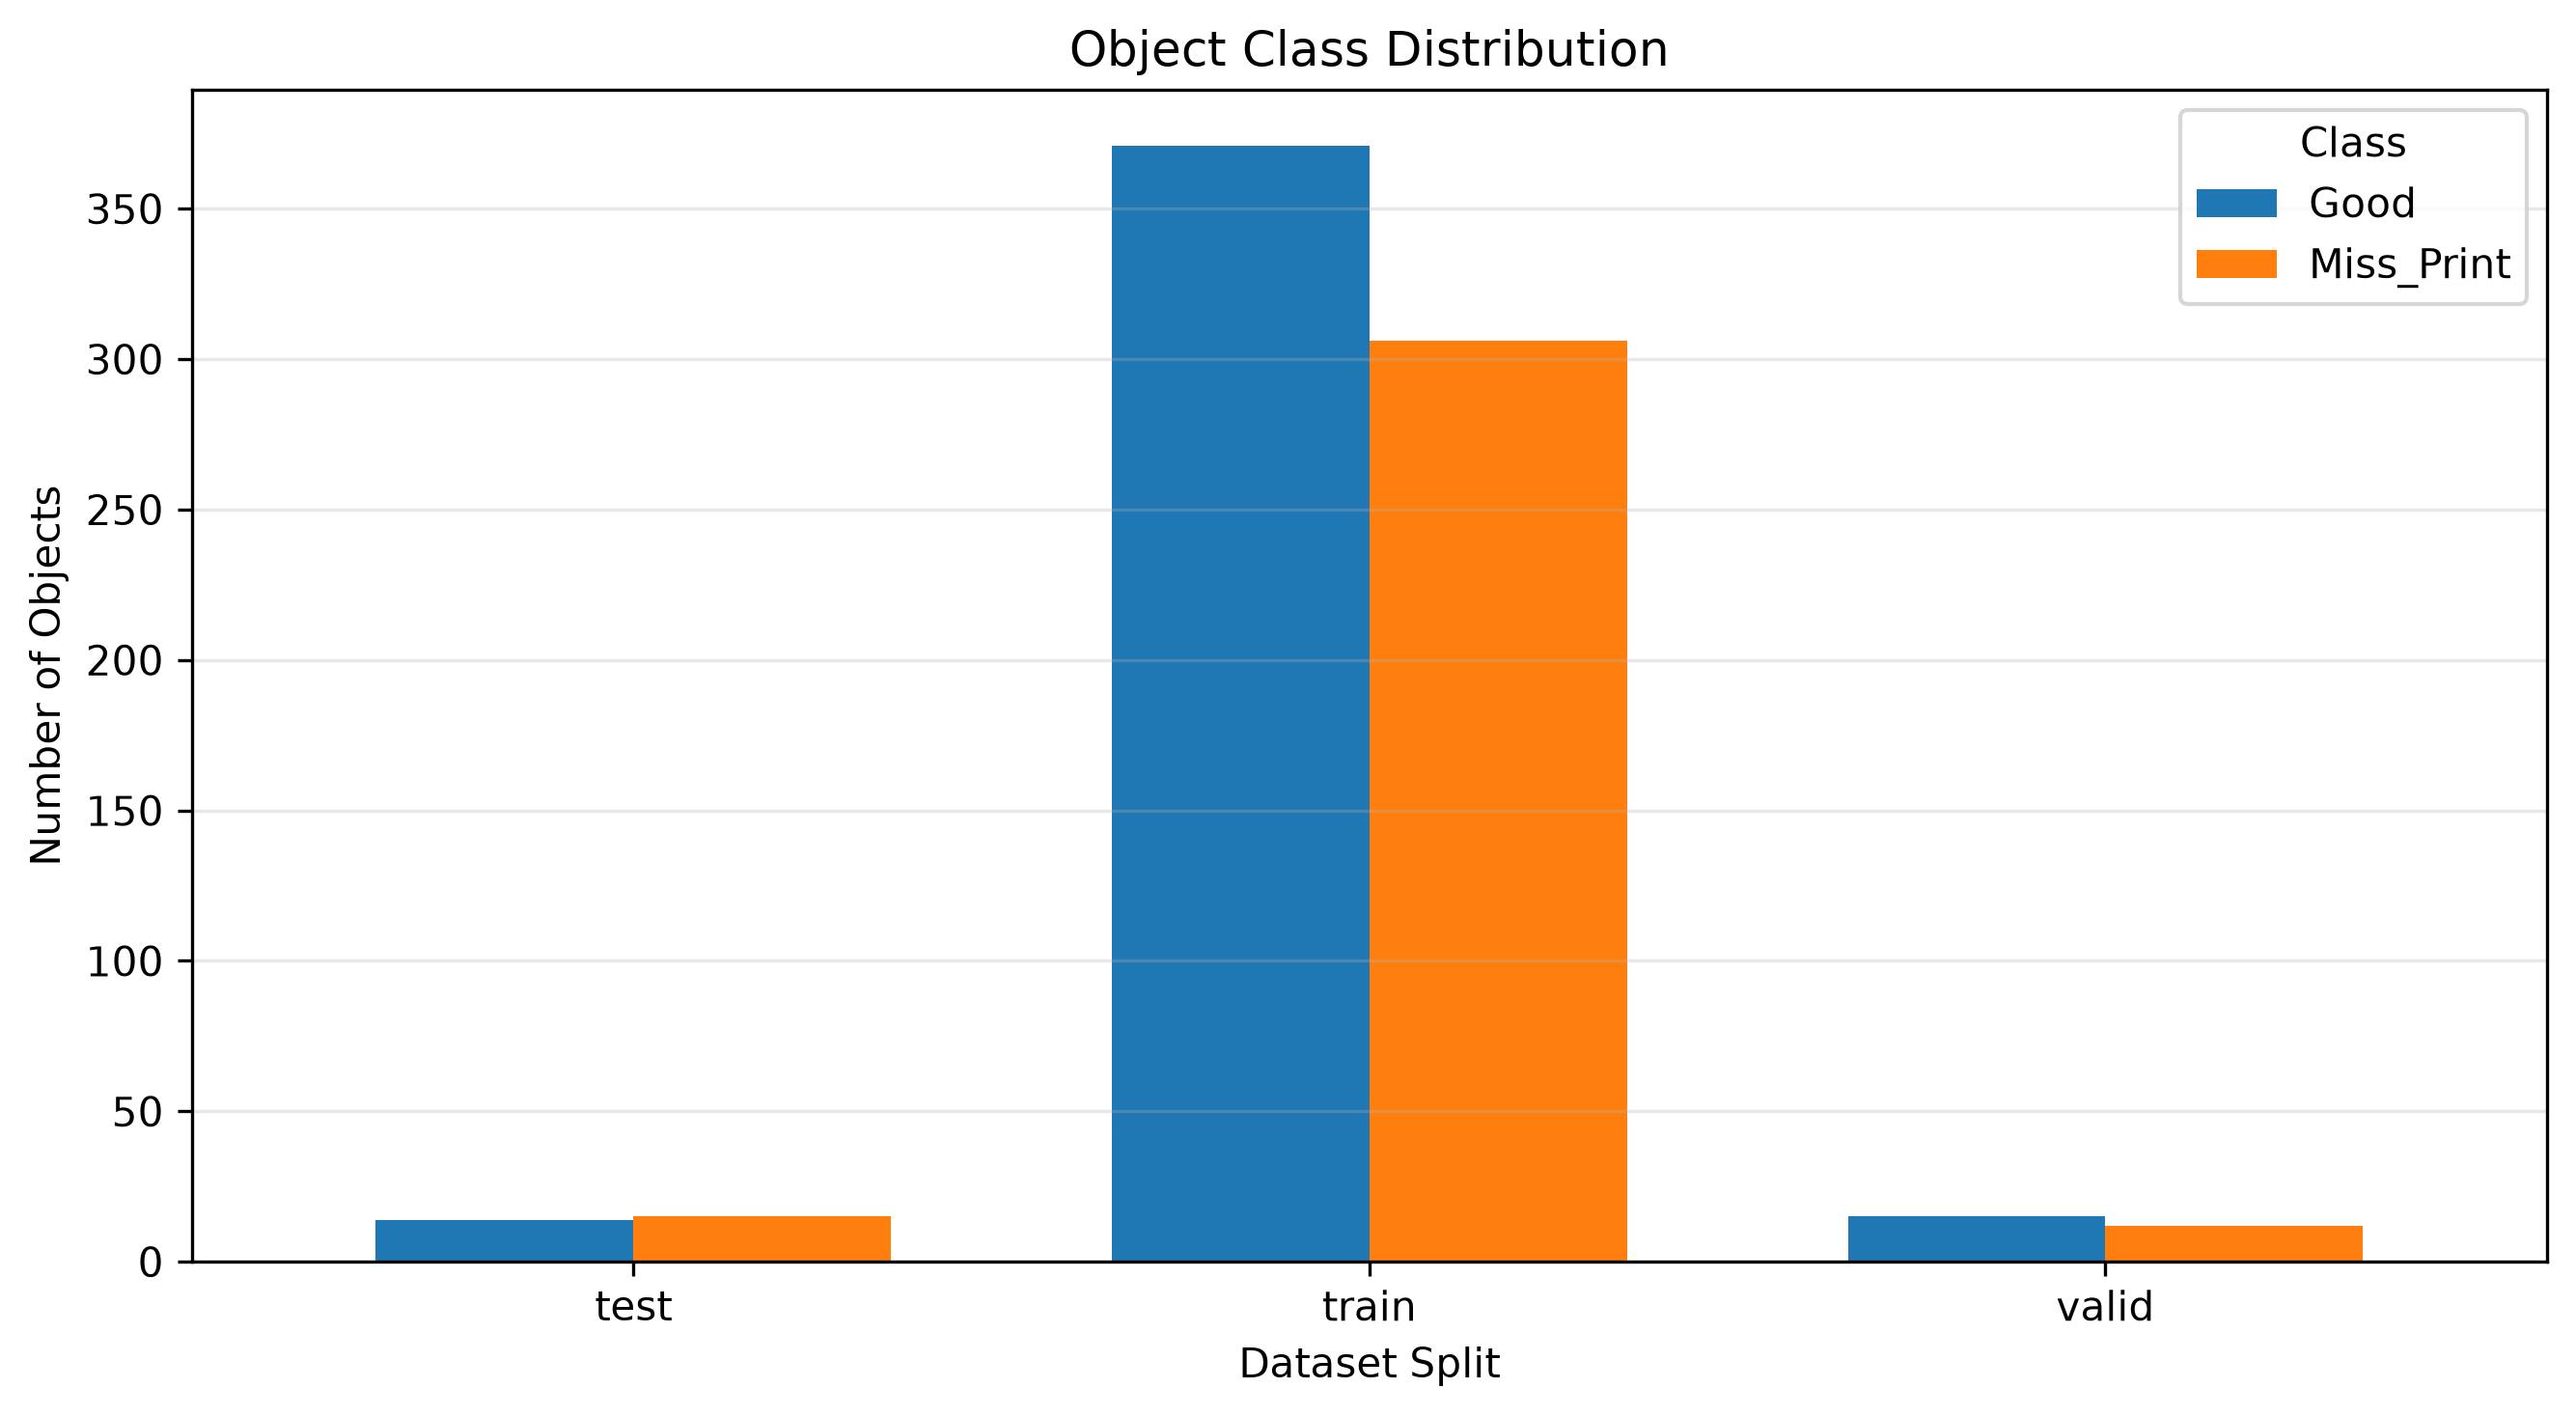
\includegraphics[width=.49\textwidth]{01_class_distribution.png}\hfill
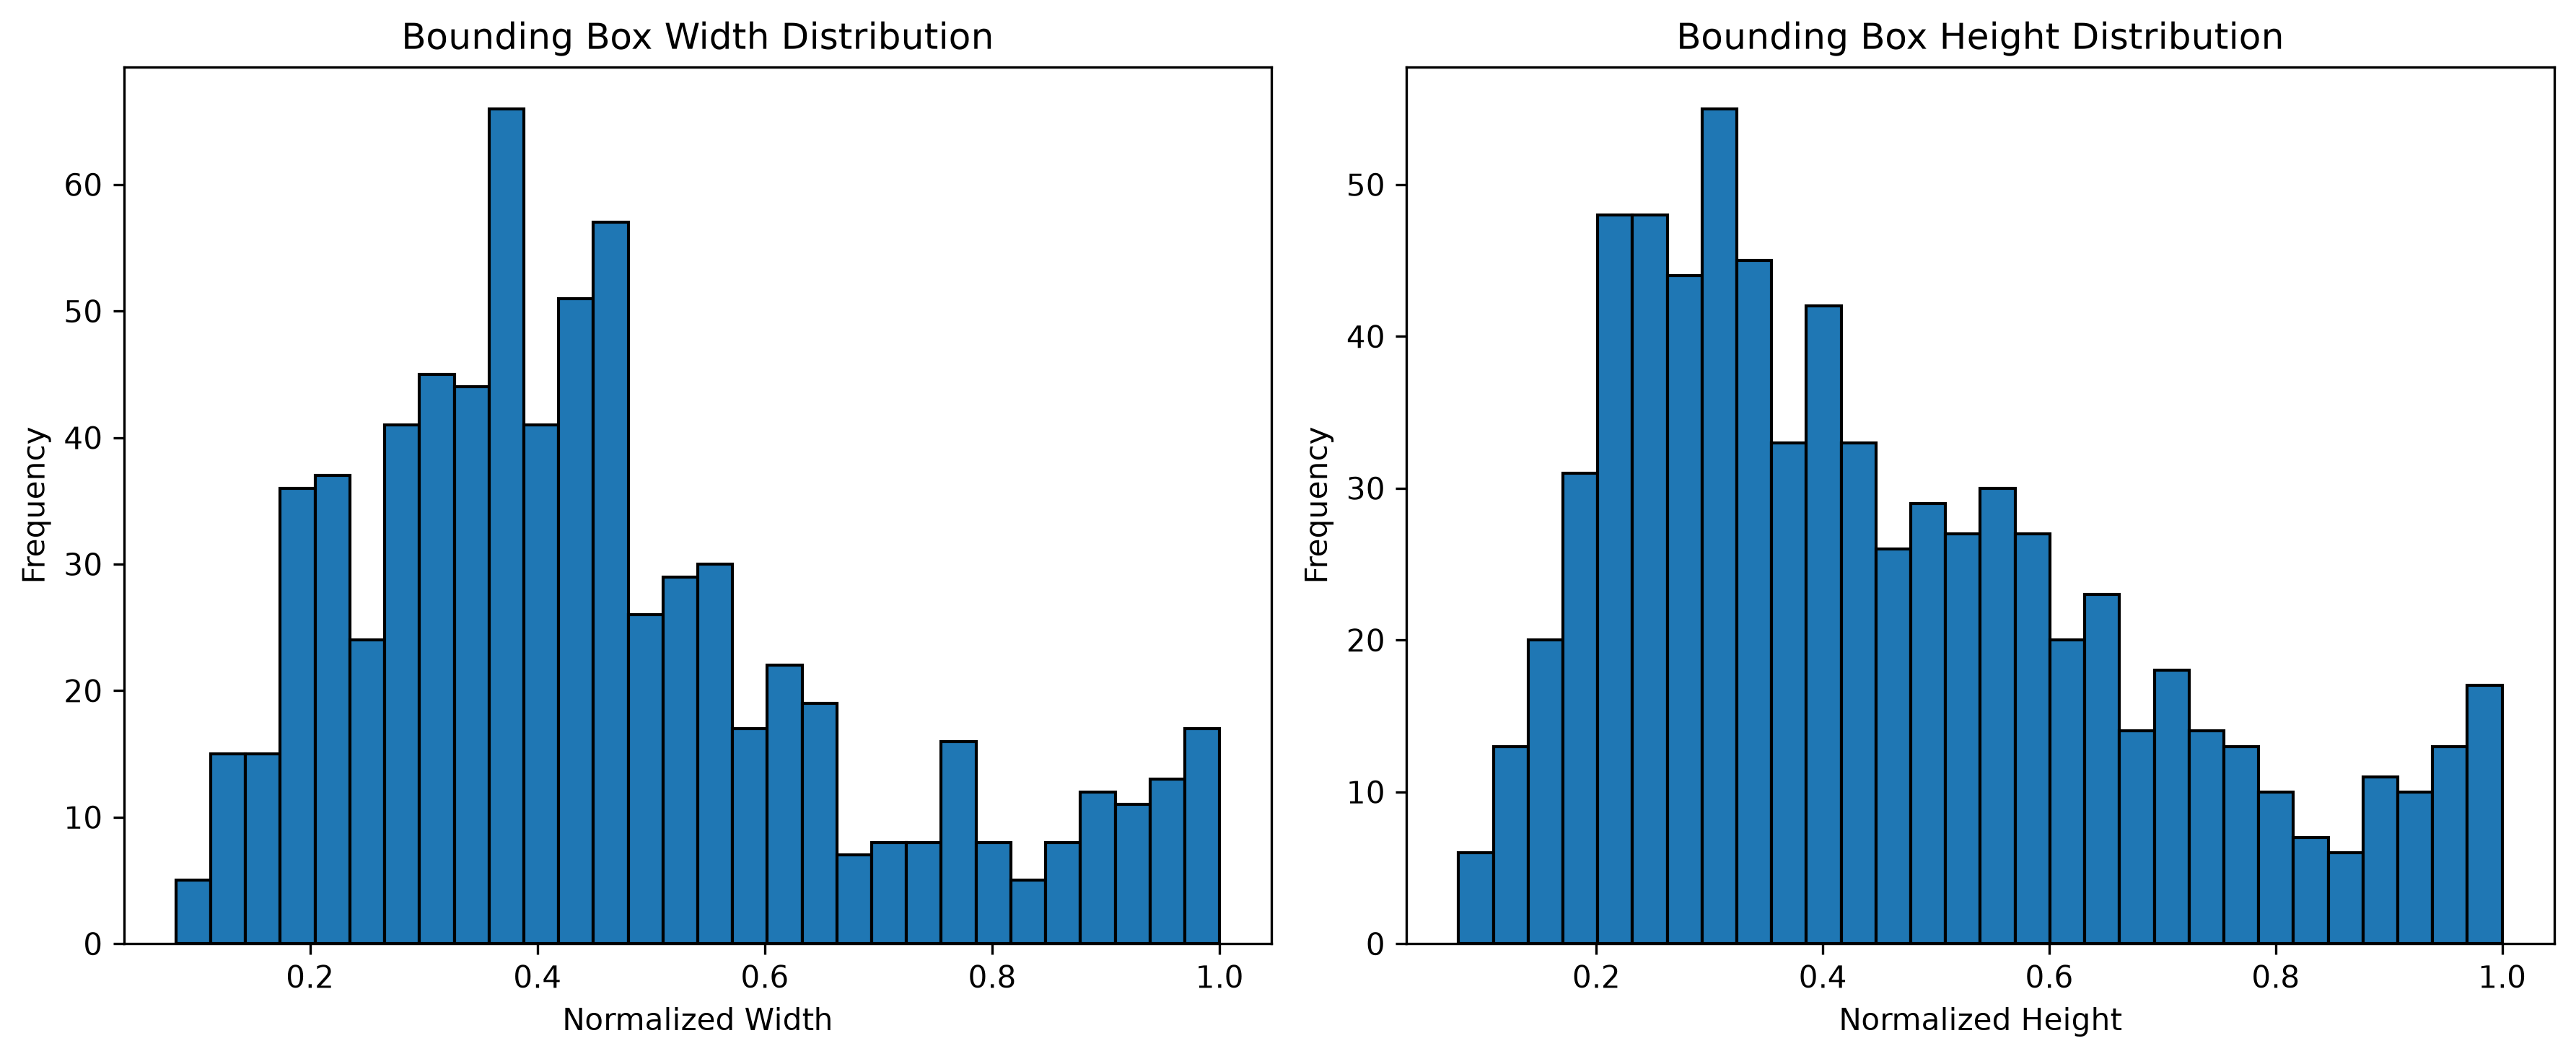
\includegraphics[width=.49\textwidth]{02_bbox_dimensions.png}\\[4pt]
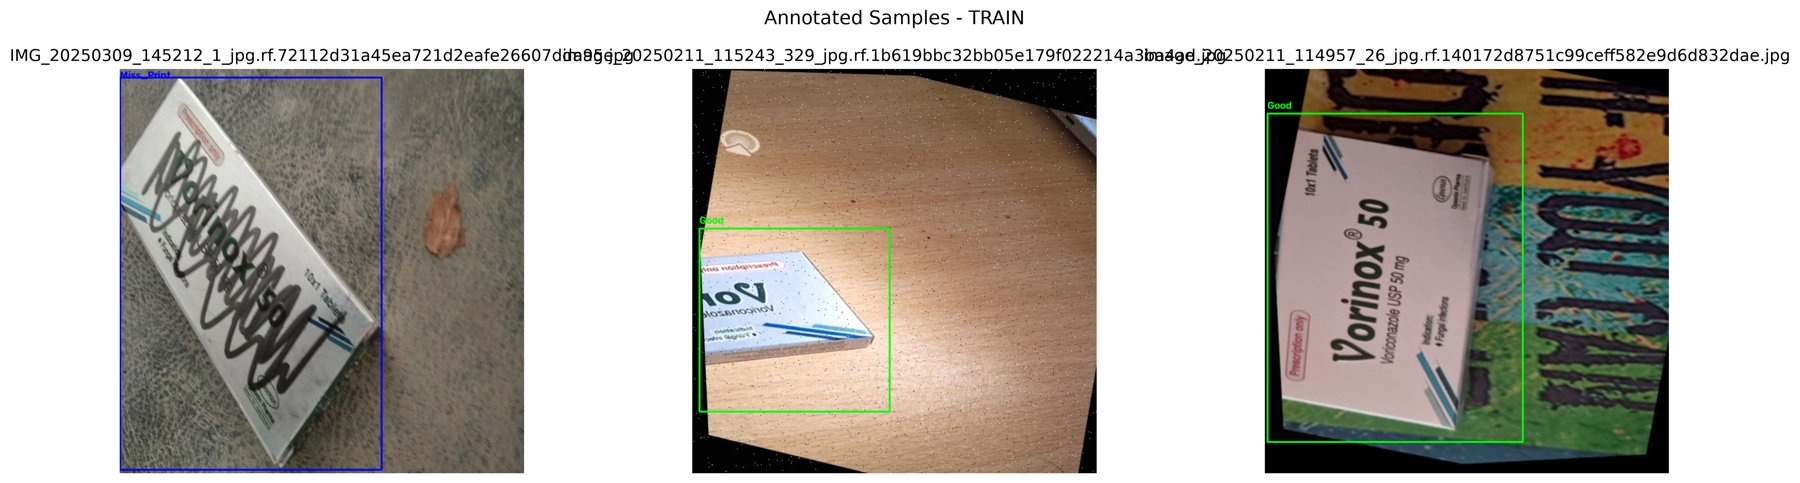
\includegraphics[width=.92\textwidth]{05_samples_train_small.jpg}
\caption{Top: object counts per class and split; normalised box width and height. Bottom: three annotated training images (one \emph{Miss\_Print}, two \emph{Good}) showing the rotation, black borders and speckle noise introduced by offline augmentation.}
\label{fig:eda}
\end{figure}

\section{Experimental set-up}\label{sec:setup}
\textbf{Recipe.} Each model started from its COCO-pretrained small checkpoint (\texttt{yolov8s.pt}, \texttt{yolo11s.pt}, \texttt{yolo12s.pt}, \texttt{yolo26s.pt}) and was fine-tuned with AdamW (learning rate 0.001, weight decay 0.0005), batch size 4, image size 640, seed 42, deterministic mode, up to 100 epochs with early stopping at patience 25. All online augmentation was disabled (mosaic, mixup, copy-paste, HSV, flips, scale, translate, rotation, shear and perspective set to zero), so the only augmentation seen is the offline Roboflow copies. The four \texttt{args.yaml} files differ only in the model name and run directory. No hyper-parameter search was performed and there is one run per model. Full settings are in Appendix~\ref{app:hp}.

\textbf{Hardware and software.} Training used an NVIDIA GeForce RTX 5060 Laptop GPU (7.9~GB), Python 3.11.3, PyTorch 2.11.0+cu128 and Ultralytics 8.4.190 on Windows 10. The test re-evaluation and bootstrap were run again on CPU in FP32 with the same Ultralytics version.

\textbf{Checkpoint choice and evaluation.} Ultralytics keeps \texttt{best.pt} by validation fitness, which for detection weights mAP@50 by 0.1 and mAP@50:95 by 0.9. The checkpoint was evaluated once on the test split with \texttt{model.val}. Precision and recall are the class means at the confidence that maximises the mean F1 curve; the F1 in the tables is the harmonic mean of those two means, as defined in the notebook. mAP@50 and mAP@50:95 follow the COCO-style averaging over IoU thresholds \cite{lin2014coco}. My CPU re-evaluation reproduced all logged test numbers to four decimals except YOLO26s mAP@50:95, which was 0.6925 against 0.6969 logged on the GPU; I report the logged value in tables and the CPU value inside the bootstrap intervals, and the difference is a reminder of how small numerical changes move a 29-box metric.

\textbf{Bootstrap.} To express test-sampling uncertainty I resampled the 21 test images with replacement 2\,000 times (seed 42) and recomputed precision, recall, mAP@50 and mAP@50:95 with Ultralytics' \texttt{ap\_per\_class} on the validator's own per-image statistics. The same resamples were used for all four models, so differences between models are paired. Intervals are 2.5th--97.5th percentiles. This captures the variance that comes from which images are in the test set; it does not capture variance between training runs or seeds, which was not measured.

\begin{figure}[H]
\centering
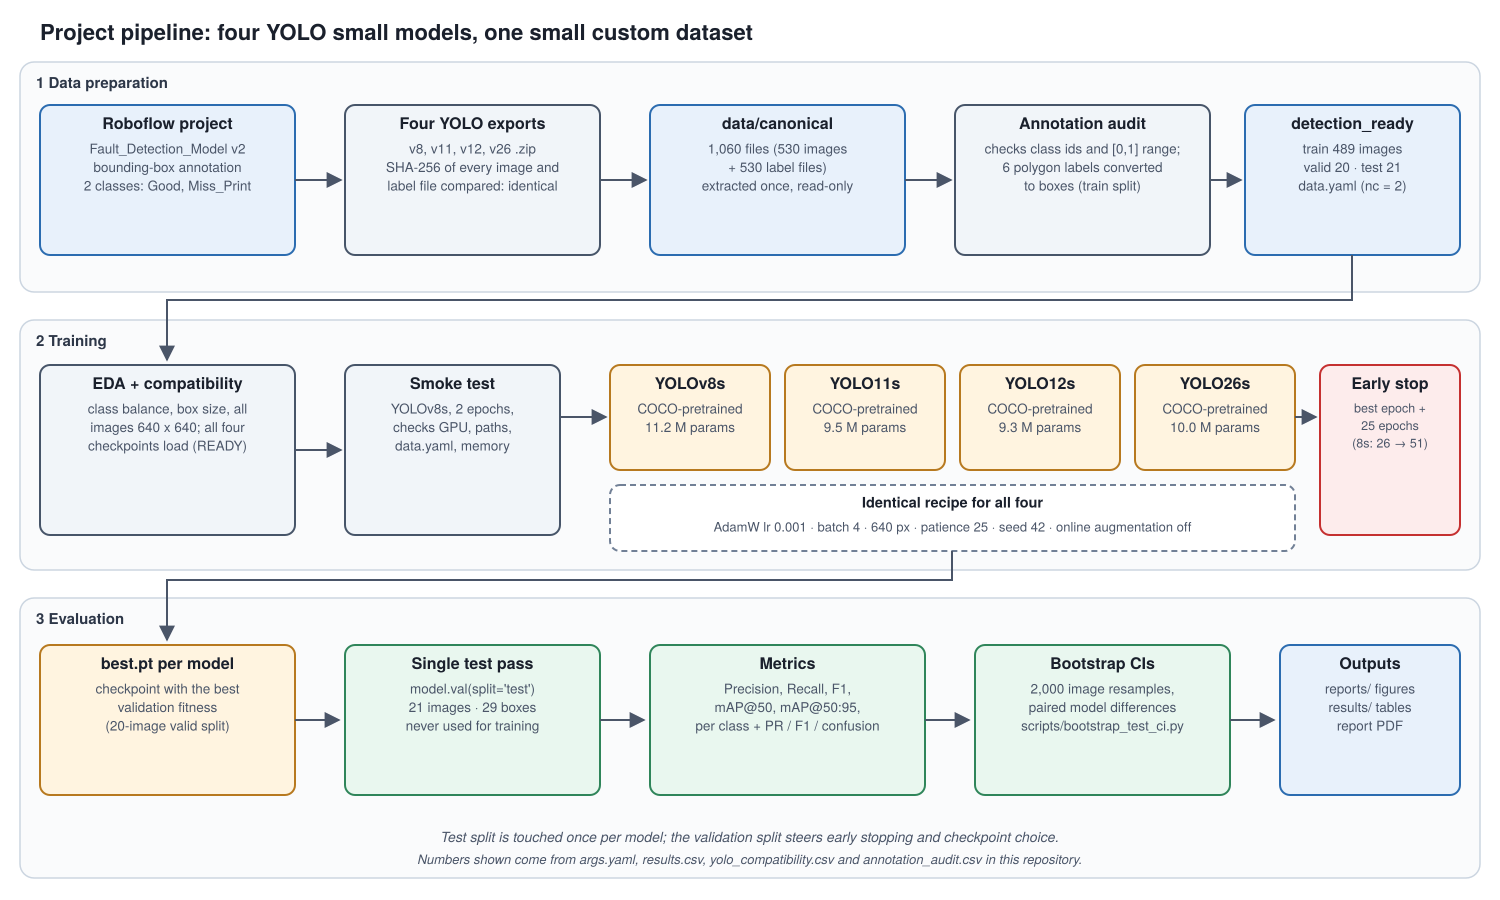
\includegraphics[width=\textwidth]{01_pipeline.png}
\caption{End-to-end pipeline of the project.}
\label{fig:pipeline}
\end{figure}

\section{Results}\label{sec:results}
\subsection{Training dynamics}
Table~\ref{tab:train} and Figure~\ref{fig:gap} show the same pattern for all four models: training losses decrease steadily, whereas validation losses fall for a few epochs and then fluctuate. The best checkpoint came at epoch 26 of 51 (YOLOv8s), 8 of 33 (YOLO11s), 47 of 72 (YOLO12s) and 39 of 64 (YOLO26s); because patience was 25, each run stopped exactly 25 epochs after its best. Validation box loss in YOLOv8s was lowest at epoch 12 (1.10) and ended at 1.31; in YOLO11s it was lowest at epoch 22 (1.04) and ended at 1.46. YOLO12s and YOLO26s ended close to their minimum (1.03 versus 0.95; 1.09 versus 1.00). In validation mAP@50:95 the same split appears: the 25 patience epochs cost YOLOv8s 0.087 and YOLO11s 0.123, but YOLO12s only 0.042 and YOLO26s 0.020.

\begin{table}[H]
\centering\small
\begin{tabular}{lrrcccrc}
\toprule
Model & Epochs & Best & Best val & Last val & Change & Val box loss & s/epoch\\
 & run & epoch & mAP$_{50:95}$ & mAP$_{50:95}$ & & min $\to$ last &\\
\midrule
YOLOv8s & 51 & 26 & 0.654 & 0.567 & $-$0.087 & 1.10 $\to$ 1.31 & 8.0\\
YOLO11s & 33 & 8  & 0.661 & 0.538 & $-$0.123 & 1.04 $\to$ 1.46 & 9.2\\
YOLO12s & 72 & 47 & 0.699 & 0.657 & $-$0.042 & 0.95 $\to$ 1.03 & 12.0\\
YOLO26s & 64 & 39 & 0.729 & 0.709 & $-$0.020 & 1.00 $\to$ 1.09 & 12.4\\
\bottomrule
\end{tabular}
\caption{Training summary from \texttt{results.csv}. ``Last'' is the final epoch before early stopping, i.e.\ 25 epochs after the best. Seconds per epoch include validation and come from a single run on a laptop GPU; they are not a controlled speed benchmark.}
\label{tab:train}
\end{table}

\begin{figure}[H]
\centering
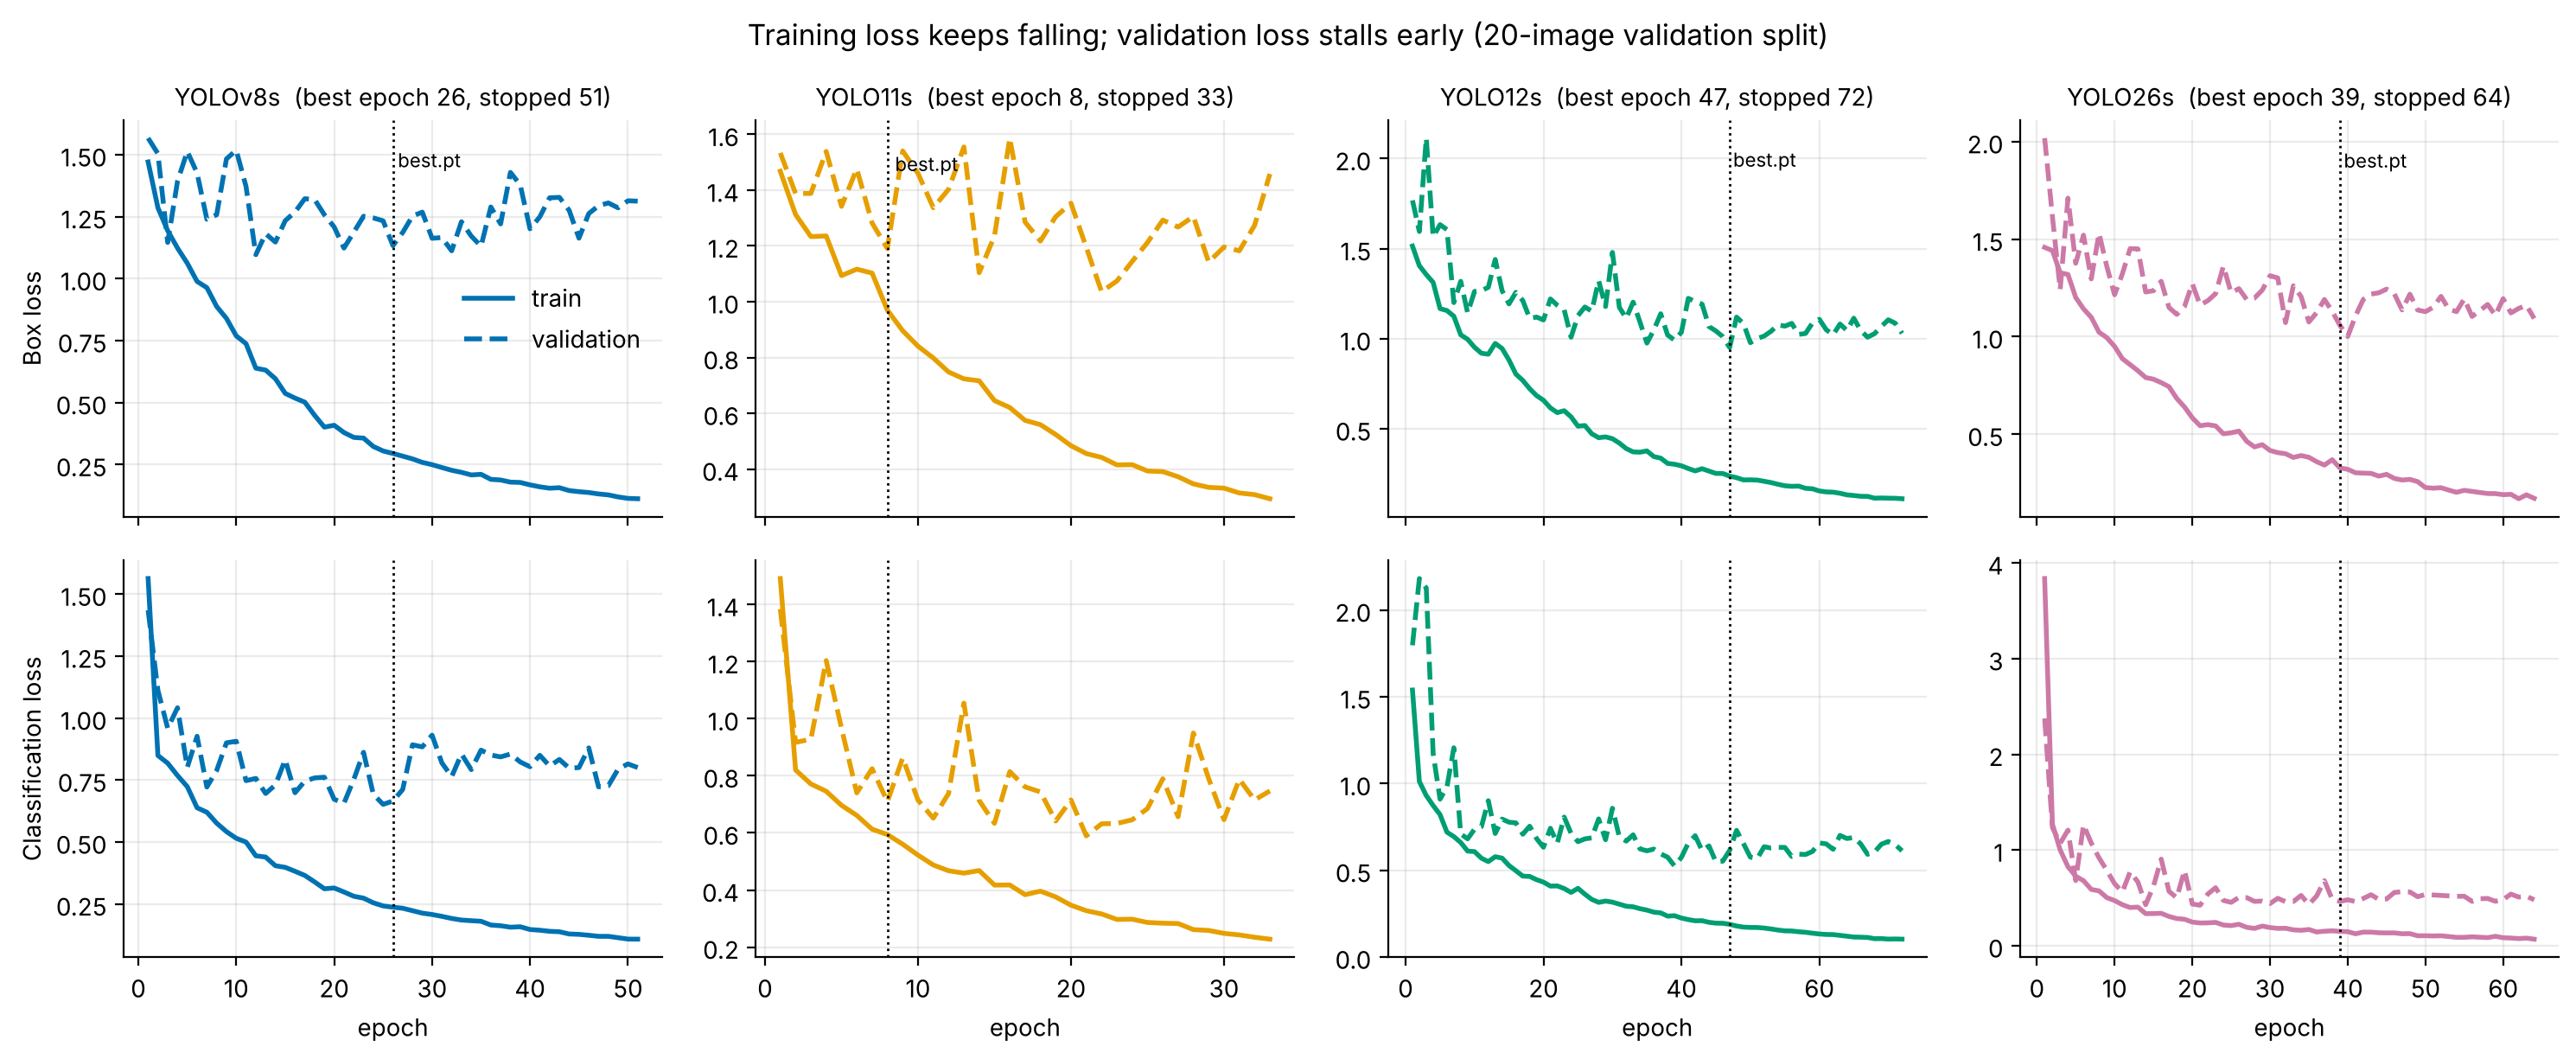
\includegraphics[width=\textwidth]{fig_A_generalisation_gap.png}
\caption{Training (solid) and validation (dashed) box and classification loss for each model; the dotted line marks the epoch kept as \texttt{best.pt}. The validation split has 20 images.}
\label{fig:gap}
\end{figure}

\begin{figure}[H]
\centering
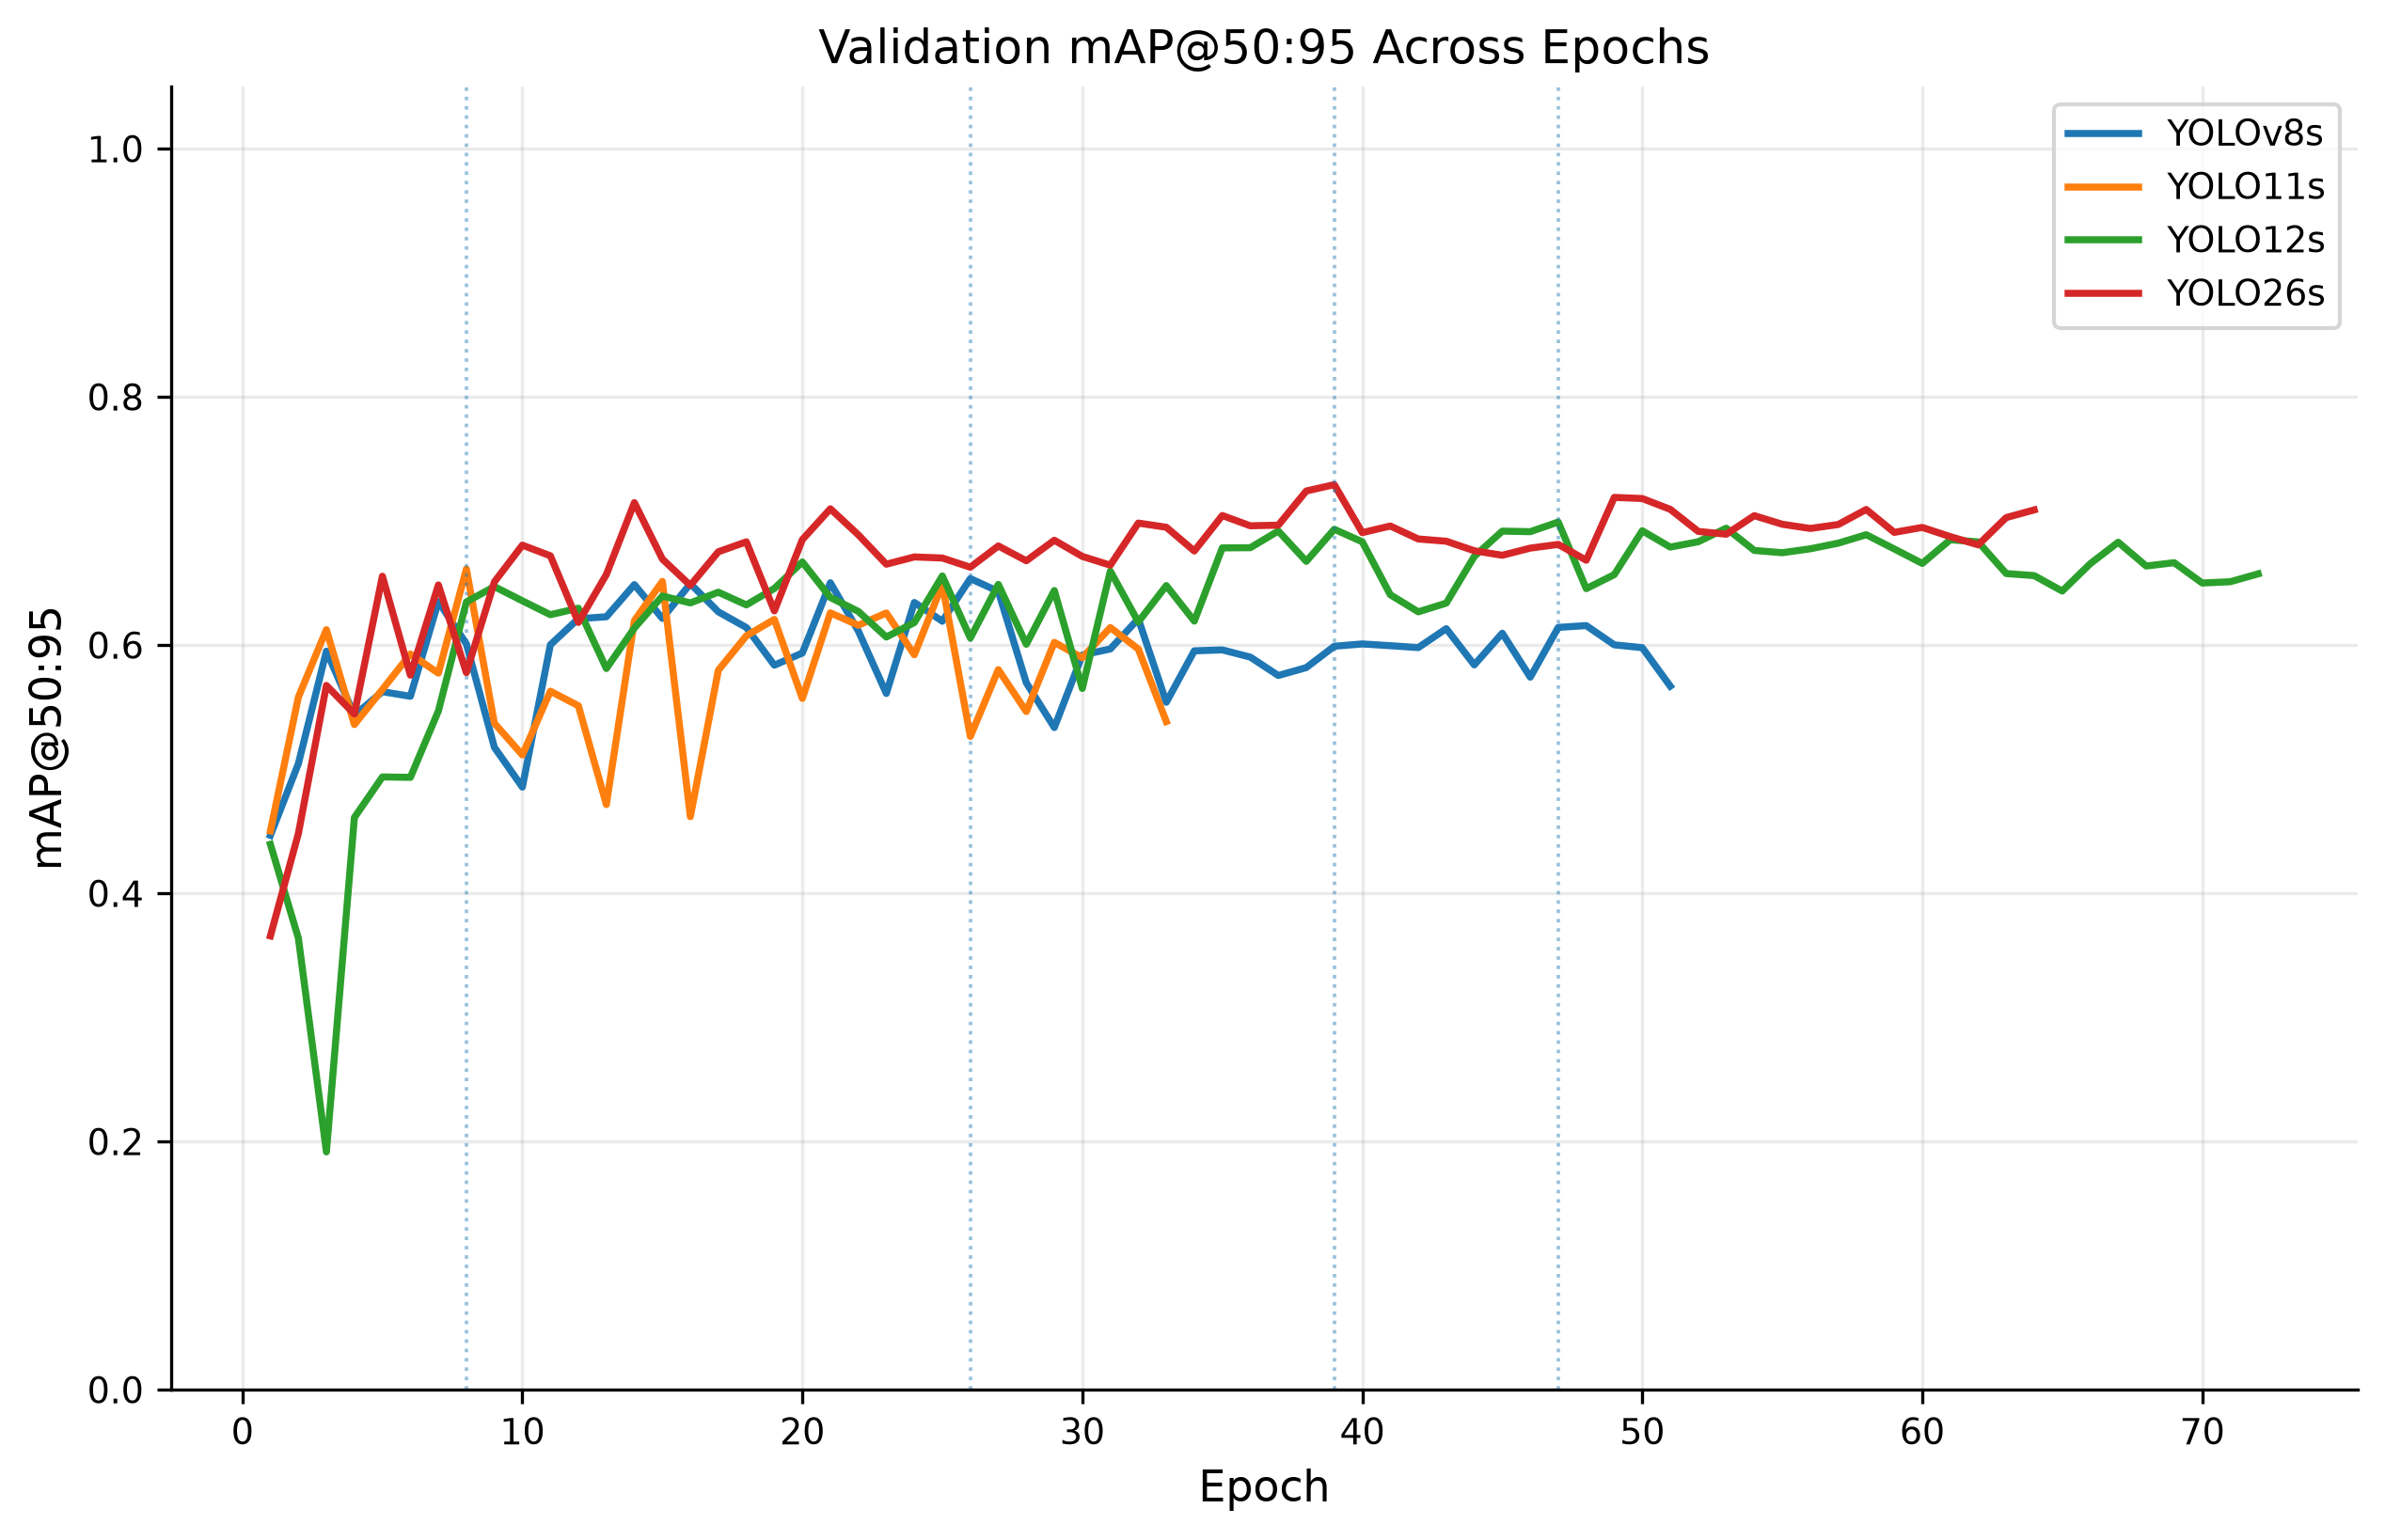
\includegraphics[width=.62\textwidth]{06_epochwise_mAP_50_95.png}\hfill
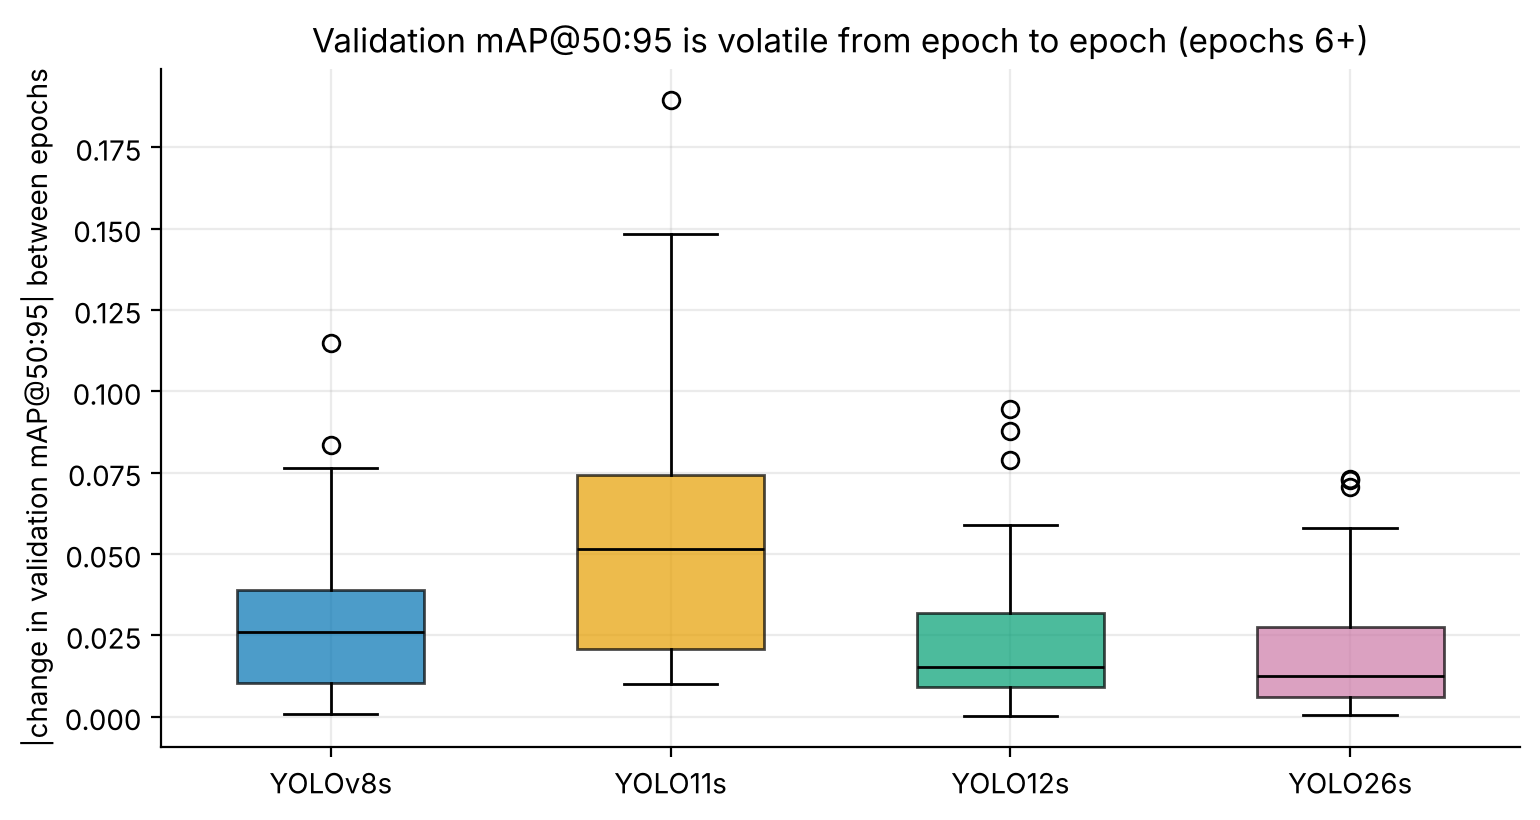
\includegraphics[width=.36\textwidth]{fig_C_val_map_volatility.png}
\caption{Left: validation mAP@50:95 per epoch (dotted lines mark each model's best epoch). Right: absolute epoch-to-epoch change after the first five epochs. Median changes were 0.026, 0.051, 0.015 and 0.012 and the largest jumps 0.115, 0.190, 0.095 and 0.073 for YOLOv8s, YOLO11s, YOLO12s and YOLO26s.}
\label{fig:vol}
\end{figure}

\subsection{Test performance}
Table~\ref{tab:test} gives the single-pass test results. By point estimate the order on mAP@50:95 is YOLO12s (0.727), YOLO26s (0.697), YOLO11s (0.625), YOLOv8s (0.583). YOLO12s reaches precision 1.000 on test, which only means that no detection above the F1-optimal threshold was a false positive on 29 boxes.

\begin{table}[H]
\centering\small
\begin{tabular}{lccccc}
\toprule
Model & Precision & Recall & F1 & mAP@50 & mAP@50:95\\
\midrule
YOLOv8s & 0.8910 & 0.8534 & 0.8718 & 0.8577 & 0.5834\\
YOLO11s & 0.8535 & 0.8772 & 0.8652 & 0.9066 & 0.6246\\
YOLO12s & \textbf{1.0000} & \textbf{0.9577} & \textbf{0.9784} & \textbf{0.9600} & \textbf{0.7271}\\
YOLO26s & 0.9492 & 0.8952 & 0.9214 & 0.9188 & 0.6969\\
\bottomrule
\end{tabular}
\caption{Test-split results (21 images, 29 boxes), values as logged by the notebook. Bold marks the highest point estimate; Section~\ref{sec:uncertainty} shows it is not always distinguishable from the runner-up.}
\label{tab:test}
\end{table}

\begin{figure}[H]
\centering
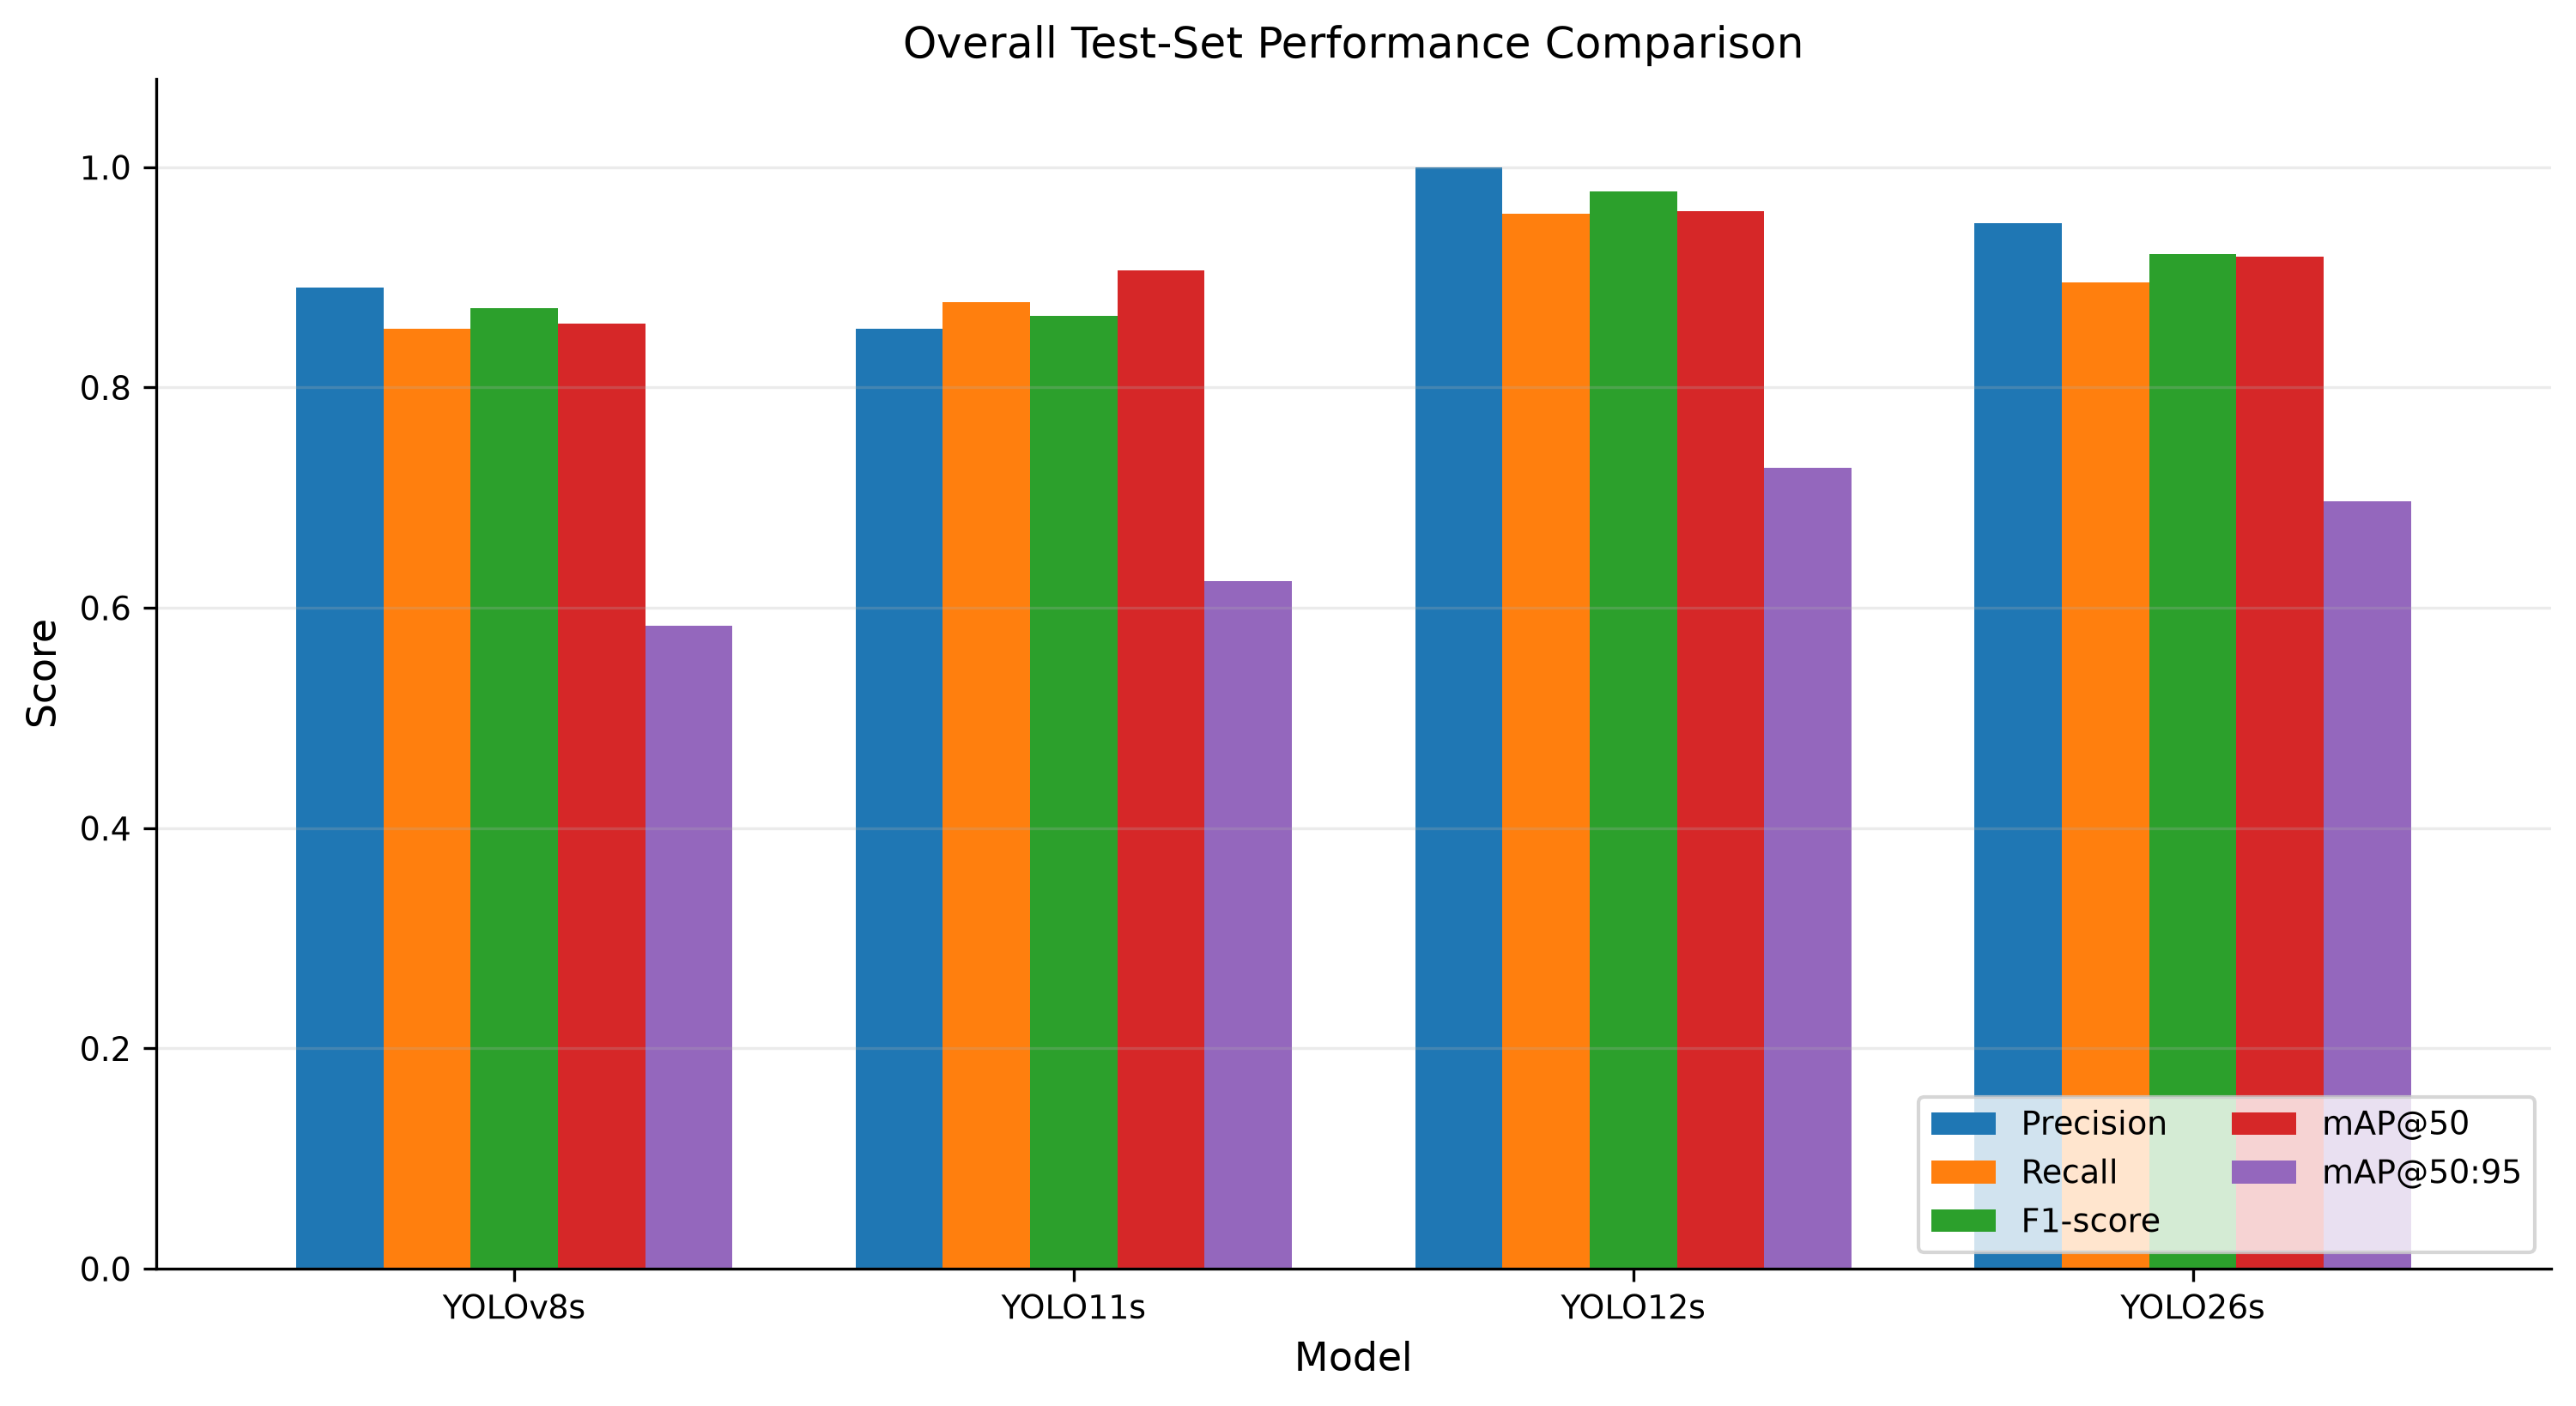
\includegraphics[width=.8\textwidth]{07_overall_test_comparison.png}
\caption{Test metrics for the four models (point estimates; see Figure~\ref{fig:forest} for uncertainty).}
\end{figure}

\subsection{Per-class results}
All four models score lower on \emph{Good} than on \emph{Miss\_Print} in mAP@50:95 (Table~\ref{tab:class}); the largest gap is YOLO26s (0.599 versus 0.795). Each class has only 14 or 15 test boxes, so per-class gaps of this size are within the sampling noise shown in Section~\ref{sec:uncertainty} and should not be read as a property of the classes.

\begin{table}[H]
\centering\small
\begin{tabular}{llccccc}
\toprule
Model & Class & Precision & Recall & F1 & mAP@50 & mAP@50:95\\
\midrule
YOLOv8s & Good       & 0.7819 & 0.7857 & 0.7838 & 0.7803 & 0.5083\\
        & Miss\_Print & 1.0000 & 0.9211 & 0.9589 & 0.9350 & 0.6585\\
YOLO11s & Good       & 0.8365 & 0.8571 & 0.8467 & 0.8920 & 0.5830\\
        & Miss\_Print & 0.8705 & 0.8972 & 0.8837 & 0.9213 & 0.6662\\
YOLO12s & Good       & 1.0000 & 0.9258 & 0.9615 & 0.9250 & 0.7105\\
        & Miss\_Print & 1.0000 & 0.9896 & 0.9948 & 0.9950 & 0.7438\\
YOLO26s & Good       & 0.9218 & 0.8571 & 0.8883 & 0.8496 & 0.5991\\
        & Miss\_Print & 0.9767 & 0.9333 & 0.9545 & 0.9879 & 0.7946\\
\bottomrule
\end{tabular}
\caption{Per-class test results (14 Good and 15 Miss\_Print boxes).}
\label{tab:class}
\end{table}

\subsection{Operating-point errors}
Metrics such as mAP hide how many boxes are involved. Table~\ref{tab:counts} counts object-level outcomes at confidence $\ge$0.25 and IoU $\ge$0.5 with class-aware matching, computed from the same validator statistics. The three best-scoring configurations all miss 3 of 29 boxes. YOLOv8s misses 6, YOLO11s has 6 false positives, and YOLO12s has none. Each of those counts is a handful of objects, which is the reason the intervals below are wide.

\begin{table}[H]
\centering\small
\begin{tabular}{lccc}
\toprule
Model & True positives & False positives & False negatives (of 29)\\
\midrule
YOLOv8s & 23 & 3 & 6\\
YOLO11s & 26 & 6 & 3\\
YOLO12s & 26 & 0 & 3\\
YOLO26s & 26 & 1 & 3\\
\bottomrule
\end{tabular}
\caption{Object-level counts on the test split at confidence $\ge$0.25 and IoU 0.5.}
\label{tab:counts}
\end{table}

\subsection{Uncertainty}\label{sec:uncertainty}
Table~\ref{tab:ci} and Figure~\ref{fig:forest} give 95\,\% bootstrap intervals. For mAP@50:95 they span 0.18 (YOLO12s) to 0.28 (YOLOv8s), i.e.\ roughly $\pm$0.09 to $\pm$0.14, and the bootstrap standard deviation is 0.046--0.073. A plain binomial argument gives the same order of magnitude: for an accuracy-like proportion $\hat p$ measured on $n=29$ independent objects, $\mathrm{SE}=\sqrt{\hat p(1-\hat p)/n}$, which is 0.056 at $\hat p=0.9$ and a 95\,\% half-width of about 0.11. Objects in the same image are not independent, so the true uncertainty is, if anything, larger.

\begin{table}[H]
\centering\small
\begin{tabular}{lcccc}
\toprule
Model & Precision & Recall & mAP@50 & mAP@50:95\\
\midrule
YOLOv8s & 0.891 [0.777, 0.993] & 0.853 [0.667, 0.967] & 0.858 [0.663, 0.990] & 0.583 [0.429, 0.713]\\
YOLO11s & 0.854 [0.769, 0.973] & 0.877 [0.720, 1.000] & 0.907 [0.755, 0.993] & 0.625 [0.502, 0.720]\\
YOLO12s & 1.000 [0.952, 1.000] & 0.958 [0.810, 1.000] & 0.960 [0.880, 0.995] & 0.727 [0.632, 0.807]\\
YOLO26s & 0.949 [0.903, 0.996] & 0.895 [0.733, 1.000] & 0.919 [0.802, 0.995] & 0.693 [0.596, 0.774]\\
\bottomrule
\end{tabular}
\caption{Test point estimate with 95\,\% percentile bootstrap interval (2\,000 resamples of 21 images). Points are from the CPU re-evaluation; they equal the logged values except YOLO26s mAP@50:95 (0.693 versus 0.697).}
\label{tab:ci}
\end{table}

\begin{figure}[H]
\centering
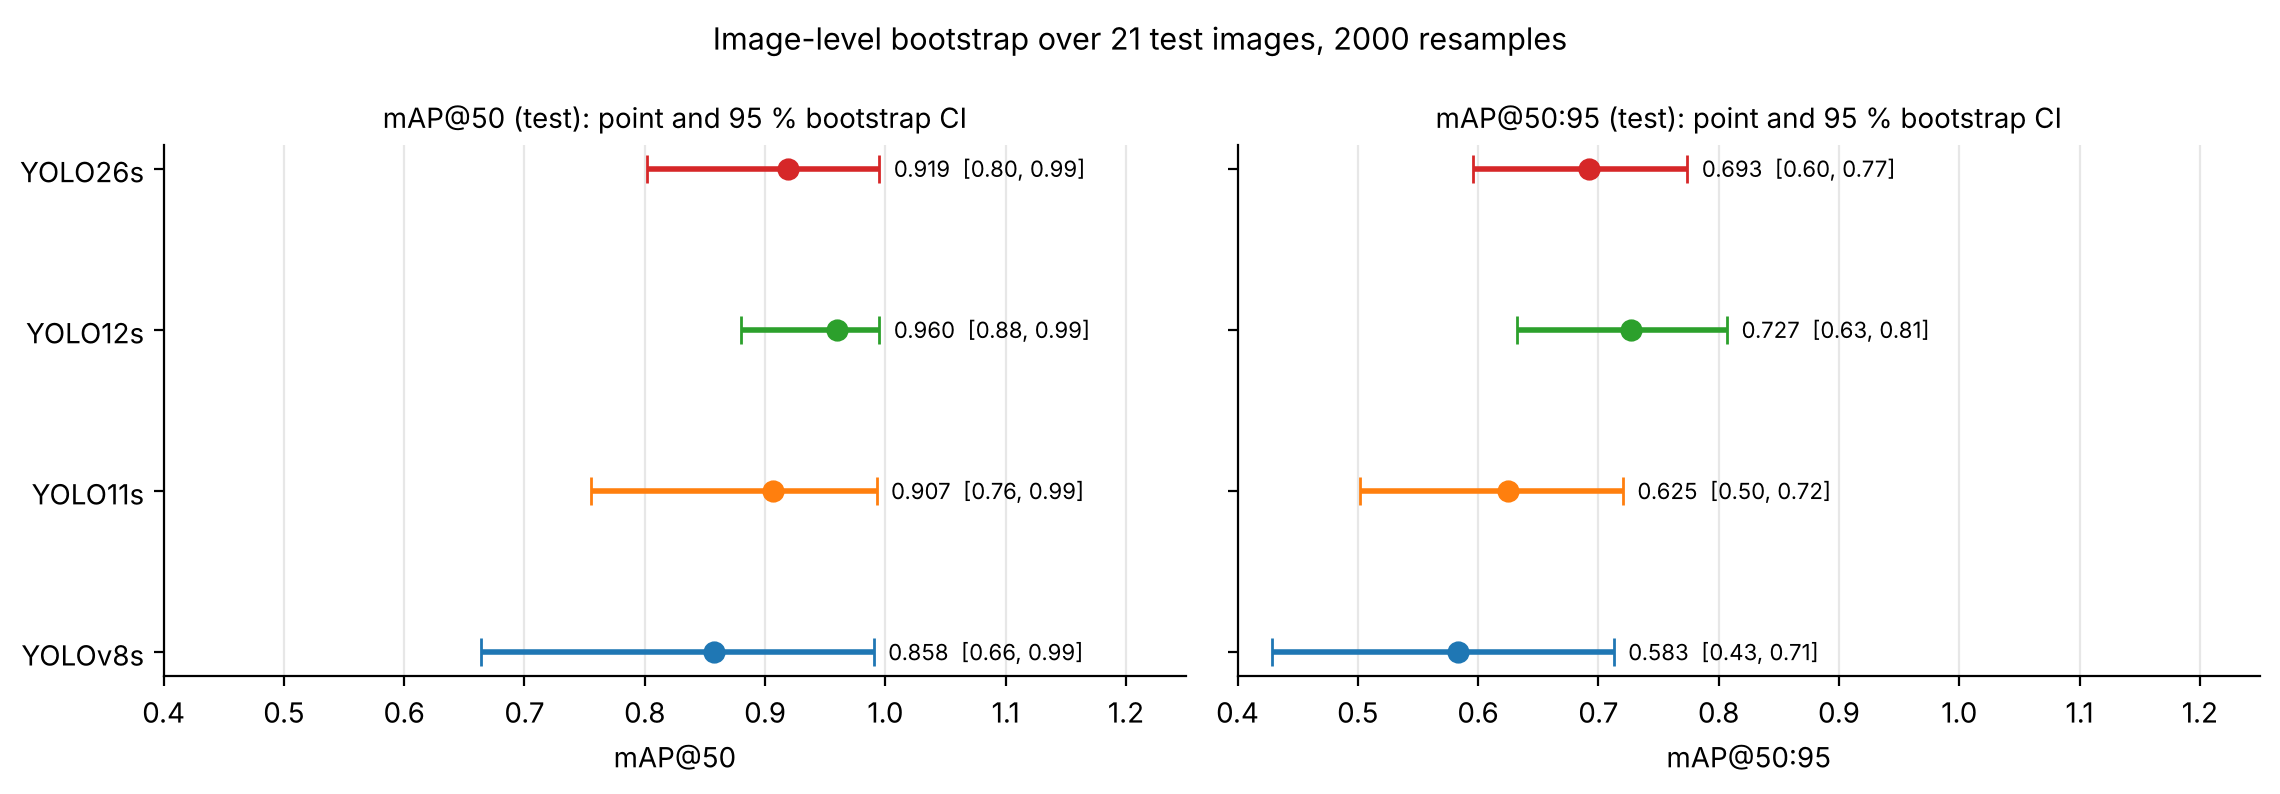
\includegraphics[width=\textwidth]{bootstrap_forest_plot.png}
\caption{Test mAP@50 and mAP@50:95 with 95\,\% bootstrap intervals.}
\label{fig:forest}
\end{figure}

Table~\ref{tab:pair} answers the question that matters for model choice. On mAP@50:95, the newer pair (YOLO12s, YOLO26s) beats the older pair (YOLOv8s, YOLO11s) in all four cross-comparisons with intervals that exclude zero, by 0.07--0.14. Inside each pair the models are not separable: YOLO12s minus YOLO26s is $+$0.035 (interval $-$0.022 to $+$0.099; YOLO12s ahead in 87\,\% of resamples), and YOLOv8s minus YOLO11s is $-$0.038 ($-$0.131 to $+$0.033). On mAP@50 only YOLO12s separates from YOLOv8s and YOLO11s; its lead over YOLO26s has an interval whose lower bound is zero (0.000 to 0.126).

\begin{table}[H]
\centering\small
\begin{tabular}{lccc}
\toprule
Comparison (A $-$ B) & Mean difference & 95\,\% interval & Excludes 0\\
\midrule
YOLOv8s $-$ YOLO11s & $-$0.038 & [$-$0.131, 0.033] & no\\
YOLOv8s $-$ YOLO12s & $-$0.145 & [$-$0.246, $-$0.059] & yes\\
YOLOv8s $-$ YOLO26s & $-$0.109 & [$-$0.203, $-$0.027] & yes\\
YOLO11s $-$ YOLO12s & $-$0.106 & [$-$0.181, $-$0.039] & yes\\
YOLO11s $-$ YOLO26s & $-$0.071 & [$-$0.127, $-$0.020] & yes\\
YOLO12s $-$ YOLO26s & $+$0.035 & [$-$0.022, 0.099] & no\\
\bottomrule
\end{tabular}
\caption{Paired bootstrap differences in test mAP@50:95 (same 2\,000 resamples for both models).}
\label{tab:pair}
\end{table}

\begin{figure}[H]
\centering
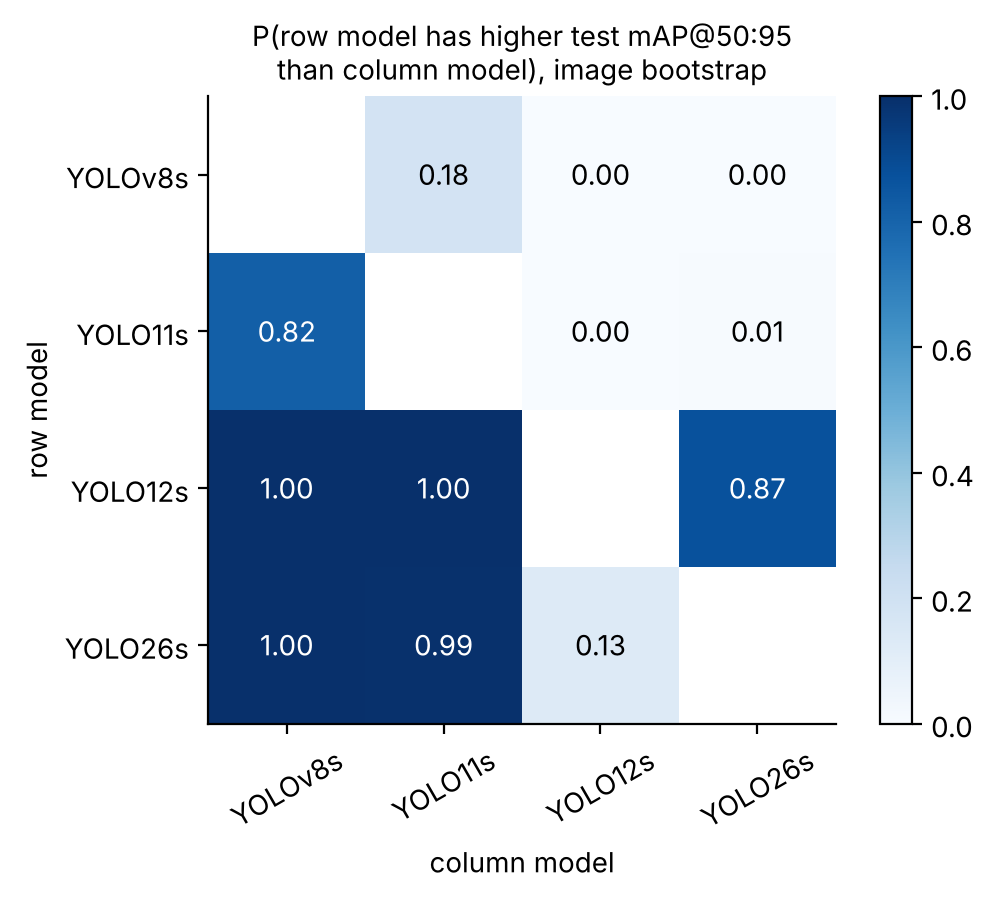
\includegraphics[width=.5\textwidth]{fig_D_pairwise_probability.png}\hfill
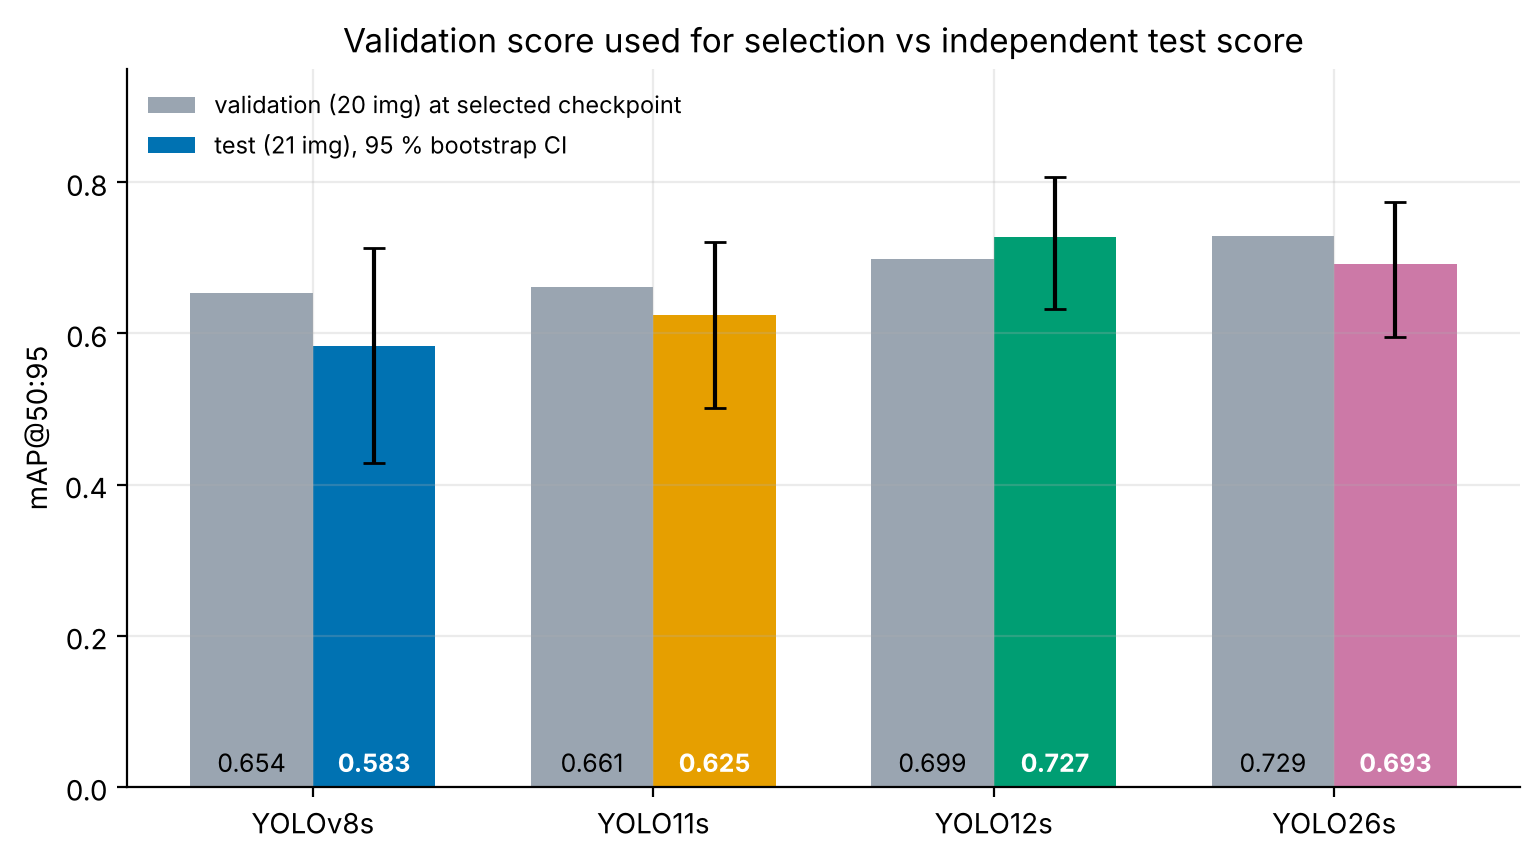
\includegraphics[width=.47\textwidth]{fig_B_val_vs_test.png}
\caption{Left: share of bootstrap resamples in which the row model has the higher test mAP@50:95. Right: validation mAP@50:95 of the selected checkpoint against the test value with its interval (test points from the CPU re-evaluation).}
\label{fig:pairwise}
\end{figure}

\textbf{What the interval does and does not cover.} The test images are the same for all models, and each model has one training run. A separation that survives resampling therefore says that the gap is not an accident of which 21 photographs were chosen. It does not say that the architecture caused the gap, because a different seed or a different early-stopping epoch could move a model by an unknown amount.

\subsection{Validation versus test}
The checkpoint was chosen on the 20-image validation split, so validation scores are expected to be optimistic. The data are consistent with that for three models and not for the fourth: test mAP@50:95 was lower than validation by 0.071 (YOLOv8s), 0.036 (YOLO11s) and 0.032 (YOLO26s, logged value) and higher by 0.028 (YOLO12s). With four models and intervals of $\pm$0.1 this is not a measurement of selection bias, only a reminder that validation numbers cannot be used as performance claims.

\section{Why the small dataset fails and why the models overfit}\label{sec:why}
\begin{figure}[H]
\centering
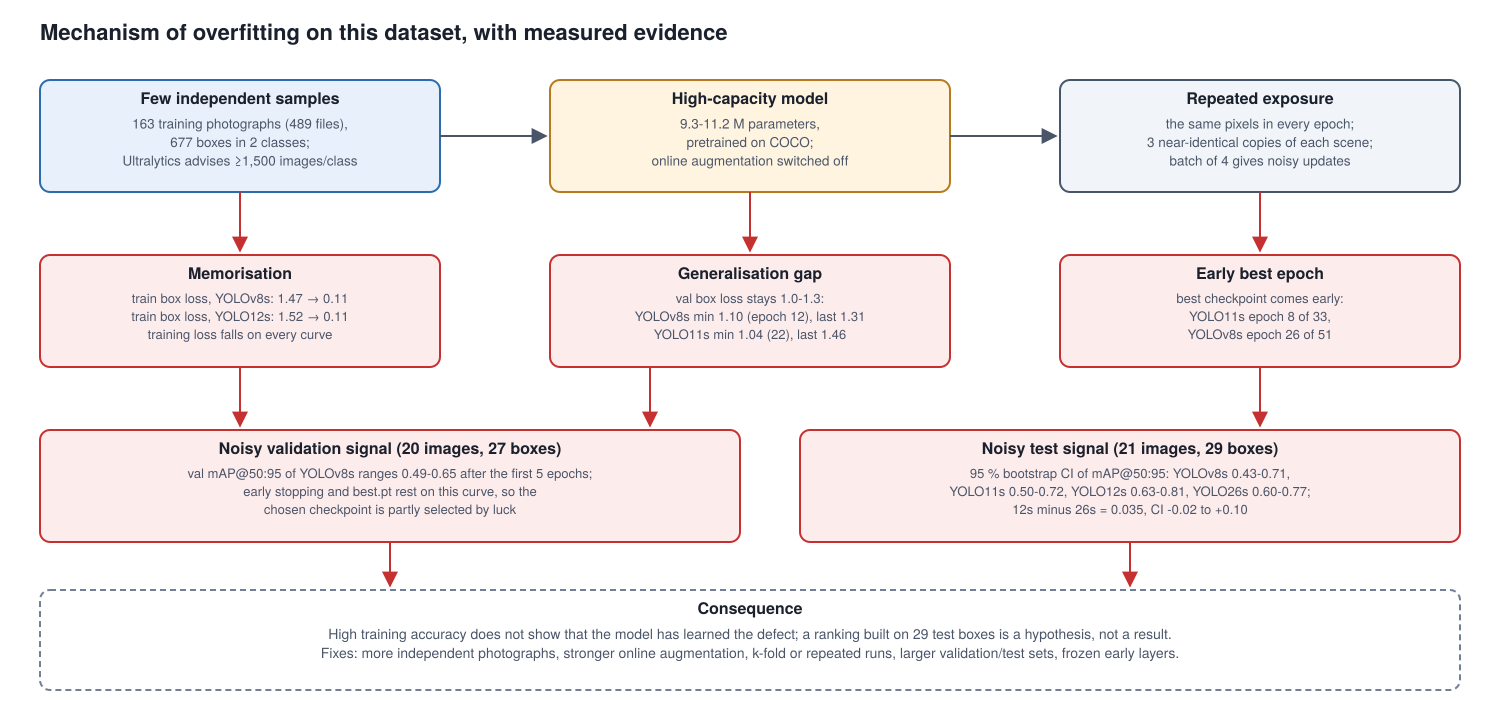
\includegraphics[width=\textwidth]{04_overfitting_mechanism.png}
\caption{Causal chain from the data and training choices to the observed symptoms, with the measured evidence in each box.}
\label{fig:mechanism}
\end{figure}

\textbf{Few independent samples.} The training split contains 677 boxes from 163 photographs, a few percent of the vendor's guideline of 10\,000 instances per class \cite{ultralytics_tips}. The two extra copies of each photograph are rotated or noisy versions of the same carton on the same background, so they add robustness to rotation and noise, not new scenes or new defects. Augmentation is known to help against overfitting \cite{shorten2019survey}, but offline copies of one scene are only a limited form of it.

\textbf{High capacity and repeated exposure.} The detectors have 9--11 million parameters; networks of this class can memorise random labels \cite{zhang2017rethinking}, so memorising 163 scenes is easy. With online augmentation set to zero (a choice made to keep the four runs identical), every epoch showed the model the same pixels. Training box loss fell from about 1.5 to 0.11 (YOLOv8s, YOLO12s), 0.17 (YOLO26s) and 0.29 (YOLO11s), while validation box loss never went below 0.95 and, after epoch 5, stayed between 0.95 and 1.6 (Figure~\ref{fig:gap}). Pretraining kept the starting point good (validation mAP@50 of 0.74--0.83 after the first epoch for every model), but it did not stop the validation signal from flattening within 8 to 47 epochs, in line with the finding that pretraining is not a regulariser \cite{he2019rethinking}. Batch size 4 additionally makes each update noisy and batch-norm statistics unreliable; I did not test this.

\textbf{Noisy selection.} Early stopping and \texttt{best.pt} depend on validation fitness measured on 27 boxes. Epoch-to-epoch jumps of 0.07--0.19 in validation mAP@50:95 (Figure~\ref{fig:vol}) are larger than most differences between epochs that the procedure tries to rank, so the selected epoch is partly chance. The same split is used both to stop and to choose, which is why its scores are optimistic.

\textbf{Noisy evaluation.} With 29 test boxes each missed object costs 3.4 recall points, and the high IoU thresholds in mAP@50:95 depend on a few well-fitted boxes. The bootstrap intervals in Table~\ref{tab:ci} are the practical expression of that limit, and a numerically tiny change (GPU against CPU arithmetic) moved YOLO26s mAP@50:95 by 0.004. The statistical point is the one made for benchmarks generally: the test set size can be the limiting factor \cite{bouthillier2021variance}.

\textbf{Why the newer models looked less overfit here.} The two models that lost least after their validation peak (YOLO12s, YOLO26s) are also the two that win on test mAP@50:95. This ordering is suggestive, not established: it rests on four runs, and I did not vary the seed. Plausible reasons that I did not test include the attention blocks and residual scaling of YOLOv12 \cite{tian2025yolov12}, the optimiser and loss changes of YOLO26 \cite{ultralytics_yolo26_vs_11}, or simply the longer runs that put the best epoch later in training.

\textbf{High mAP@50, lower mAP@50:95.} Test mAP@50 of 0.86--0.96 against mAP@50:95 of 0.58--0.73 means the detectors find the carton but place boxes less tightly at strict IoU. With large, isolated objects (median box covering 16\,\% of the image) that gap says more about box-tightness conventions and label precision than about recognition of the defect, and it is the metric most affected by annotation noise.

\section{Threats to validity and limitations}\label{sec:limits}
\begin{itemize}[leftmargin=1.4em,itemsep=2pt]
  \item \textbf{One run per model, one seed.} Training variance is unknown, so no architectural ranking can be claimed.
  \item \textbf{Test set of 21 photographs and 29 boxes.} Intervals are about $\pm$0.1; percentile bootstrap intervals are themselves approximate at this size and are skewed for metrics bounded near 1.
  \item \textbf{Validation reused for stopping and checkpoint choice.} Validation scores are optimistic; only the test numbers are independent of that choice, and they were evaluated once.
  \item \textbf{Online augmentation disabled.} This removes the main regulariser for all four models, so absolute scores are probably lower than a tuned recipe would give. Whether the ranking would survive default augmentation was not tested, and no augmented baseline was run.
  \item \textbf{No from-scratch or frozen-backbone baseline.} I cannot say how much of the performance comes from COCO pretraining.
  \item \textbf{One product and one defect family.} Sampled images show the same carton type with dark scribble-like marks on \emph{Miss\_Print} examples. Generalisation to other products, print defects, lighting or cameras is untested, and the report cannot say whether the 204 photographs cover the intended deployment.
  \item \textbf{Photograph count is inferred} from file-name stems, not from the original Roboflow project.
  \item \textbf{Speed was not benchmarked.} Seconds per epoch (Table~\ref{tab:train}) are from single runs on one laptop GPU; no inference-latency or edge-device test was made.
  \item \textbf{Documentation sources.} The YOLO26 description relies on vendor documentation and on one secondary review; the Ultralytics dataset-size guidance is a heuristic from the YOLOv5 pages.
\end{itemize}

\section{What to do next}\label{sec:next}
In order of expected value per hour of work:
\begin{enumerate}[leftmargin=1.4em,itemsep=2pt]
  \item \textbf{Collect more independent photographs, not more augmented copies.} Add new cartons, surfaces, lighting and defect instances. Grow validation and test to at least 100 images each so a single object moves recall by under one point.
  \item \textbf{Re-split by photograph with cross-validation.} Five-fold cross-validation over the 204 photographs (augmenting only inside the training folds) uses every photograph for testing once and gives a variance estimate per model.
  \item \textbf{Repeat each run with at least three to five seeds}, report mean and spread, and only then compare architectures.
  \item \textbf{Switch online augmentation on} (mosaic, scale, HSV, flips where physically valid) and compare against the off setting for at least one model; consider freezing early backbone layers for the very smallest data.
  \item \textbf{Use a held-out set the selection never touches} and report intervals with every metric, as done here.
  \item \textbf{Measure what the deployment needs}: inference latency on the target device, false-positive rate on defect-free frames, and robustness to lighting and viewpoint.
\end{enumerate}

\section{Conclusion}
On 21 test photographs, YOLO12s had the highest point estimates (mAP@50 0.960, mAP@50:95 0.727), followed by YOLO26s, YOLO11s and YOLOv8s. After resampling, only a coarse statement survives: the two newer models score higher than the two older ones on mAP@50:95, and the order within each pair is not resolved. The same models also lost the least validation accuracy after their peak, which points to milder overfitting but rests on one run each. The dataset itself, 163 independent training photographs and 20 and 21 for validation and test, is too small to rank four similar detectors and too small for validation scores to be trusted. Adding independent photographs and repeating runs would change this far more than switching architecture.

\section*{Reproducibility}
The repository contains the notebook, the exact training arguments, per-epoch logs, best checkpoints, all result tables, the bootstrap script (\texttt{scripts/bootstrap\_test\_ci.py}) and a leakage-audit script. The dataset images are not redistributed; \texttt{data/README.md} explains how to rebuild them from the Roboflow project.

\section*{Items for the author to confirm before publishing}
\begin{itemize}[leftmargin=1.4em,itemsep=1pt]
  \item The labelling rule that separates \emph{Good} from \emph{Miss\_Print}, who annotated, and how many products and cameras are in the data.
  \item The number of original photographs and the augmentation recipe in the Roboflow project (here inferred from file names and sample images).
  \item Whether the dataset may be shared publicly, and under which licence.
  \item AI-assistance disclosure: this report was drafted with Claude (Anthropic) from the author's notebook, logs and files; every number was computed from those files or from the re-evaluation described above, and should be checked by the author.
\end{itemize}

\appendix
\section{Training settings}\label{app:hp}
\begin{table}[H]
\centering\small
\begin{tabular}{ll}
\toprule
Setting & Value (identical for all four models)\\
\midrule
Task / data & detect; \texttt{data/detection\_ready/data.yaml} (nc $=$ 2)\\
Epochs / patience & 100 / 25\\
Batch / image size & 4 / 640\\
Optimiser & AdamW, lr0 0.001, lrf 0.01, momentum 0.937, weight decay 0.0005\\
Warm-up & 3 epochs (momentum 0.8, bias lr 0.1)\\
Loss gains & box 7.5, cls 0.5, dfl 1.5 (not used by YOLO26)\\
Augmentation & mosaic, mixup, copy-paste, HSV, flips, scale, translate, degrees, shear, perspective all 0\\
Other & seed 42, deterministic, AMP on, workers 2, save\_period 10, close\_mosaic 10\\
Pretrained weights & \texttt{yolov8s.pt}, \texttt{yolo11s.pt}, \texttt{yolo12s.pt}, \texttt{yolo26s.pt}\\
\bottomrule
\end{tabular}
\caption{Settings read from the four \texttt{args.yaml} files, which differ only in model and directory names. In the Ultralytics release used here the \texttt{auto\_augment} and \texttt{erasing} entries are listed in the files but apply to classification only according to the notebook's configuration.}
\end{table}

\section{Additional test-set figures}
\begin{figure}[H]
\centering
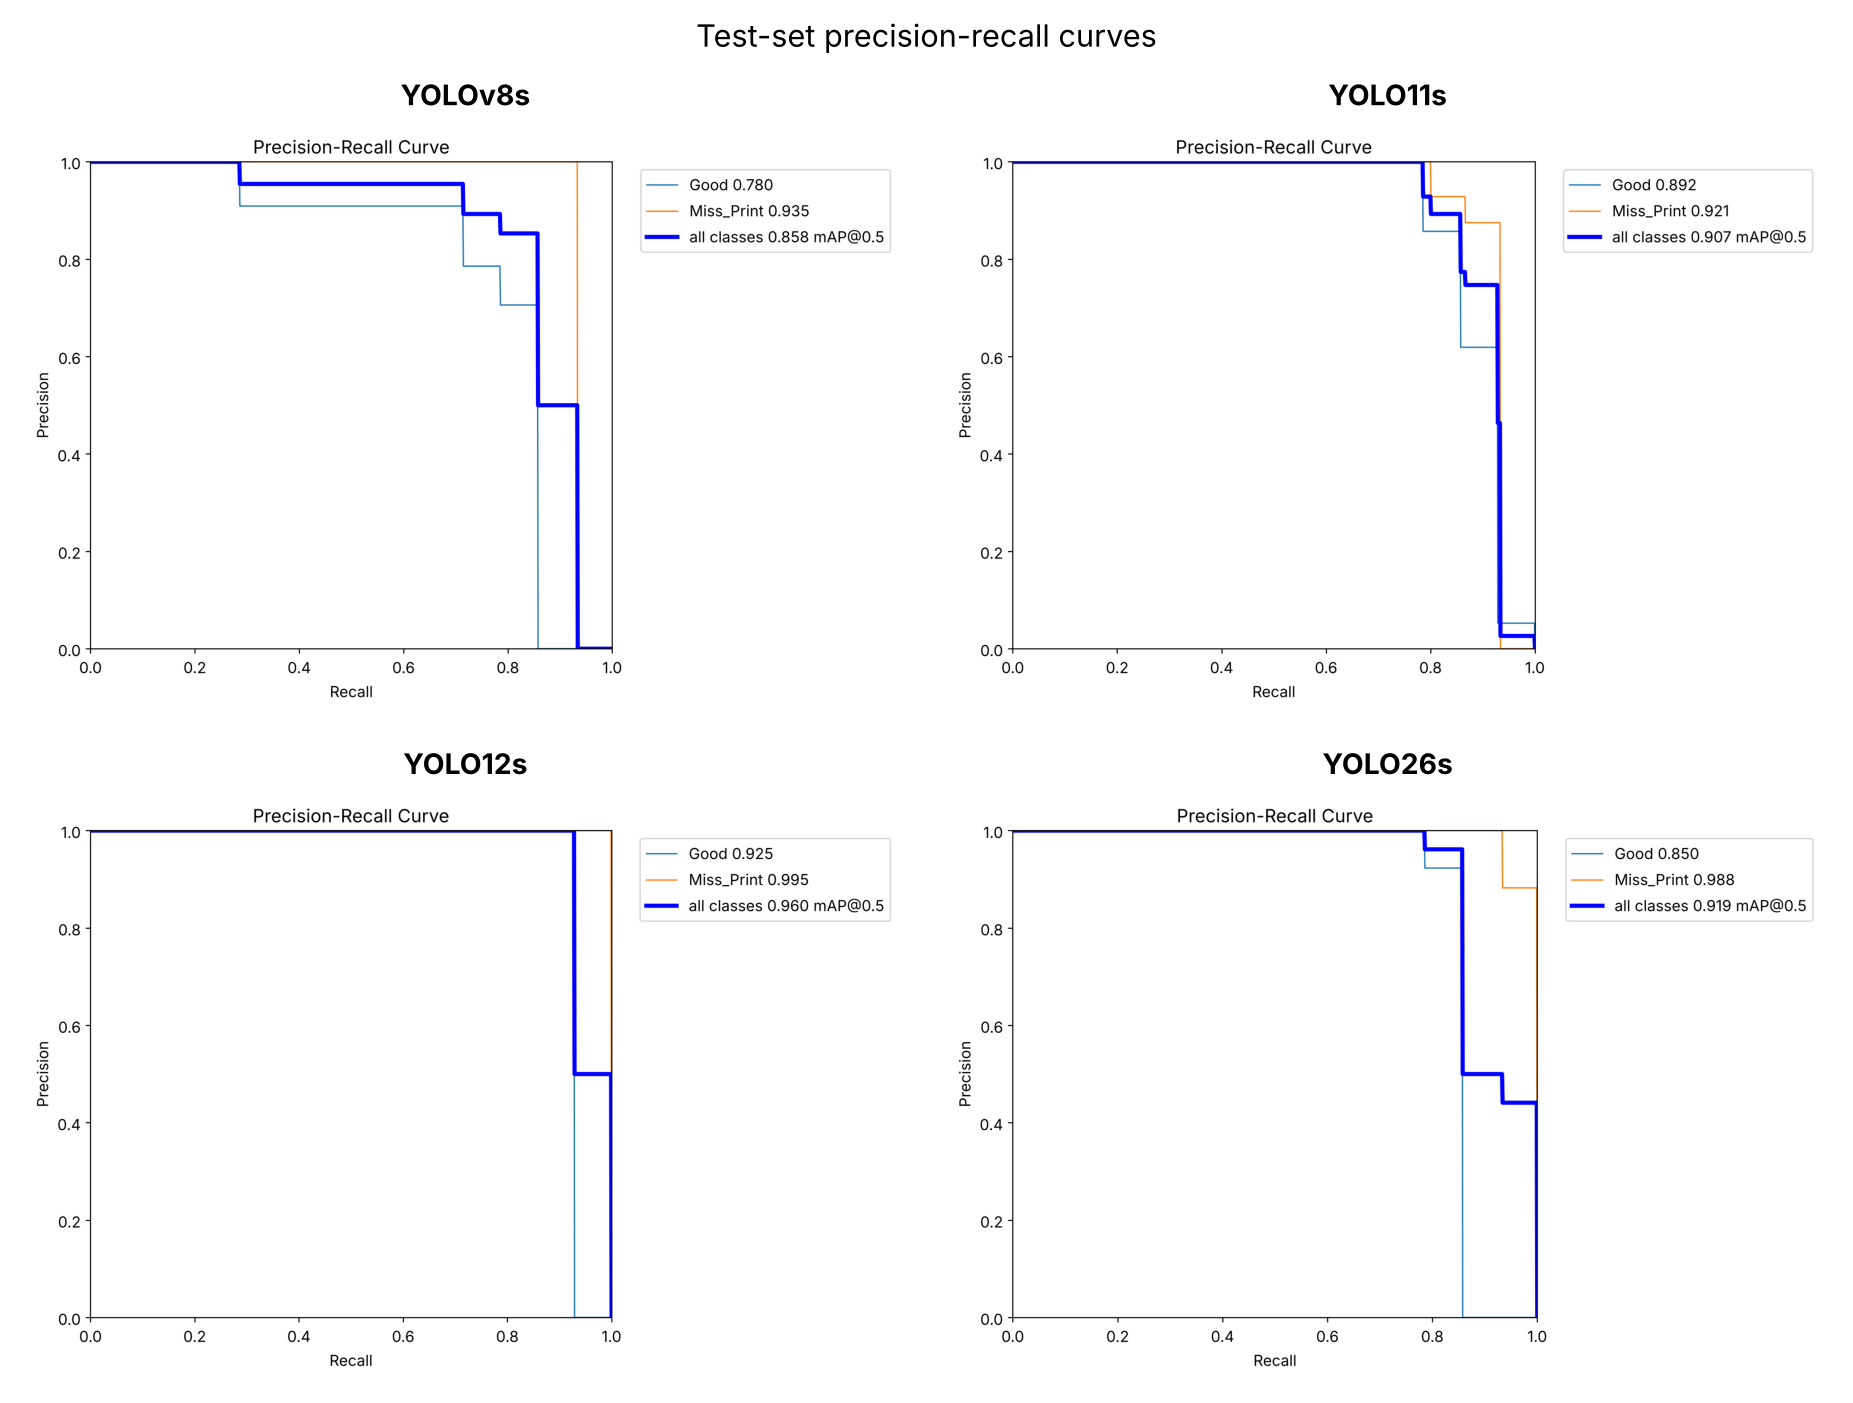
\includegraphics[width=.92\textwidth]{test_pr_curves_2x2.png}
\caption{Precision--recall curves on the test split (re-generated on CPU with the same checkpoints).}
\end{figure}
\begin{figure}[H]
\centering
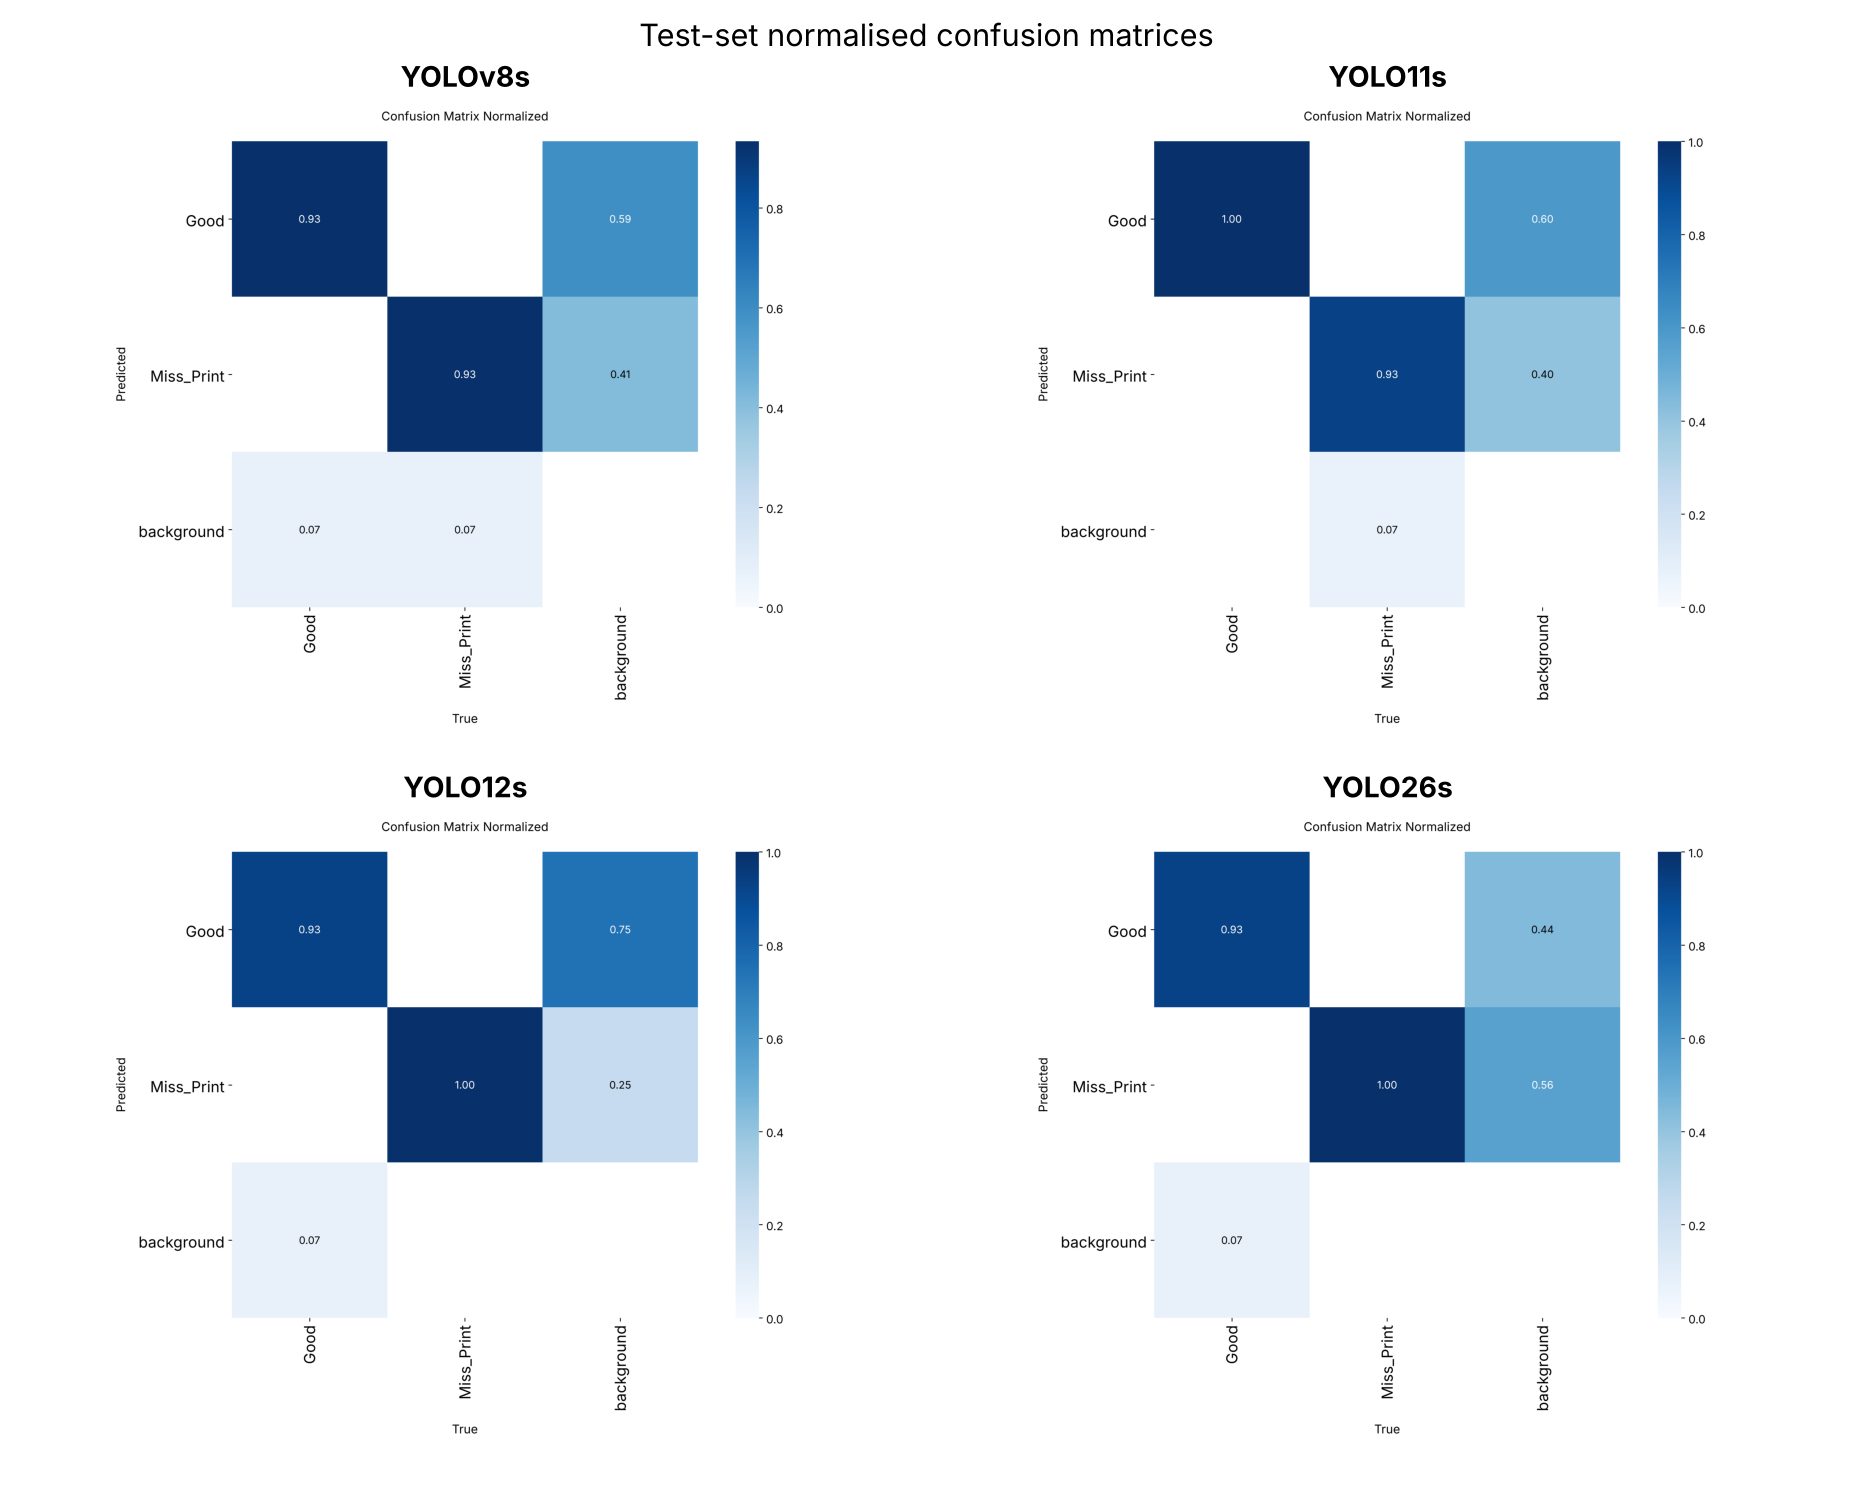
\includegraphics[width=.92\textwidth]{test_confusion_2x2.png}
\caption{Normalised confusion matrices on the test split. The background column counts detections that match no ground-truth box and is sensitive to the confidence threshold used for the matrix.}
\end{figure}

\section{Source ledger}
Items opened and read during the work, with what was taken from each. Entries marked ``partly'' could not be read in full.
\begin{itemize}[leftmargin=1.4em,itemsep=1pt,font=\small]
  \item Ultralytics, tips for best training results (read): dataset-size guidance, epochs, pretrained weights \cite{ultralytics_tips}.
  \item Ultralytics, YOLO26 versus YOLO11 (read): YOLO26 changes, parameters, FLOPs, COCO mAP \cite{ultralytics_yolo26_vs_11}.
  \item Chakrabarty, YOLO26 analysis (partly: first part verbatim, remainder via a model summary): architecture description \cite{chakrabarty2026yolo26}.
  \item Tian et al., YOLOv12 (read): contributions, YOLOv12-S figures, FlashAttention limitation \cite{tian2025yolov12}.
  \item Ultralytics, YOLO11 versus YOLOv8 (read): C3k2, C2PSA, parameters, COCO mAP \cite{ultralytics_yolo11_vs_v8}.
  \item Zhang et al. (read abstract/page) \cite{zhang2017rethinking}; He et al. (read full text) \cite{he2019rethinking}; Bouthillier et al. (read) \cite{bouthillier2021variance}.
  \item Shorten and Khoshgoftaar (DOAJ record only; publisher PDF redirected) \cite{shorten2019survey}.
  \item Roboflow documentation, image augmentation (read): augmentation applied to training images only \cite{roboflow_augmentation}.
  \item Ultralytics configuration page (partly: patience, close\_mosaic, optimiser defaults verified; augmentation defaults not verified, so none are quoted) \cite{ultralytics_cfg}.
  \item arXiv abstract pages for YOLO \cite{redmon2015yolo} and COCO \cite{lin2014coco}: authors and titles confirmed; venues are not stated on those pages and are omitted.
\end{itemize}

\bibliographystyle{unsrt}
\bibliography{references}

\end{document}
